\makeatletter
\let\@starttocorig\@starttoc
\makeatother%%

\documentclass[10pt,xcolor={usenames},fleqn,mathserif,serif]{beamer}

%%%Usefull link
%tikz-equations:
%http://www.wekaleamstudios.co.uk/posts/creating-a-presentation-with-latex-beamer-equations-and-tikz/

%% colors
\definecolor{bittersweet}{rgb}{1.0, 0.44, 0.37}
\definecolor{brilliantlavender}{rgb}{0.96, 0.73, 1.0}
\definecolor{antiquefuchsia}{rgb}{0.57, 0.36, 0.51}
\definecolor{violetw}{rgb}{0.93, 0.51, 0.93}
\definecolor{Veronica}{rgb}{0.63, 0.36, 0.94}
\definecolor{atomictangerine}{rgb}{1.0, 0.6, 0.4}
\definecolor{darkgray}{rgb}{0.66, 0.66, 0.66}
\definecolor{brightcerulean}{rgb}{0.11, 0.67, 0.84}
\definecolor{cadmiumorange}{rgb}{0.93, 0.53, 0.18}
\definecolor{ochre}{rgb}{0.8, 0.47, 0.13}
\definecolor{midnightblue}{rgb}{0.1, 0.1, 0.44}
\definecolor{lemon}{rgb}{1.0, 0.97, 0.0}
\definecolor{grey}{rgb}{0.7, 0.75, 0.71}
\definecolor{amber}{rgb}{1.0, 0.75, 0.0}
\definecolor{almond}{rgb}{0.94, 0.87, 0.8}
\definecolor{bf}{RGB}{88, 86, 88}
\definecolor{bb}{RGB}{177, 177, 177}
\definecolor{keyword}{rgb}{0.25, 0.25, 0.28}

%%%%%%%%%%%%%%%%%%%%%%%%%%%%%%%%%%% importa pacchetti
\usepackage{usepkg}
%%%%%%%%%%%%%%%%%%%%%%%%%%%%%%%%%%% Funzioni generali
\usepackage{functions}
%http://tex.stackexchange.com/questions/246/when-should-i-use-input-vs-include
\newcommand{\setmuskip}[2]{#1=#2\relax} %%problem usinig mu with calc (req by mathtools) loaded
\usepackage{sources}
%\usepackage{length}
%%%%%%%%%%%%%%%%%%%%%%%%%%%%%%%%%%% Funzioni per questo file main
\usepackage{mathOp}

%%tikz sources

%%%%
\def\status{coazione}
\def\keeptrying{coazione}
\usepackage{LocalF}
%%%%%%%%%%%%%%%%%%%%%%%%%%%%%%%%%
\usepackage{beamersetup}
%% Titolo
\title{Interazioni fondamentali}

% Let's get started
\begin{document}


\begin{filecontents}{coulombdistant.tex}


\begin{figure}
    \centering
\begin{tikzpicture}
    \coordinate (c) at (0,0) ;
\draw[->] (3,0) node[above] {$\vec{k_i}= \frac{\vec{p_i}}{\hbar}$} -- (0,0) ;
\draw[->] (0,0)--(0.5,-0.5);
\draw (0.3,-0.2) node  {$\vec{x}'$};
\draw[->]  (0,0)--(-2,0.5);
\draw (-0.2,0.2) node[above] {$\vec{x}$};
\draw[->] (0.5,-0.5) --(-2,0.5) node[above] {$\Pelectron$};
\draw (-1.3,-0.2) node[above] {$\vec{x}-\vec{x'}$};
\draw[black,fill=gray,opacity=0.4, rounded corners=1mm] (c) \irregularcircle{1cm}{2mm};

\draw (0.5,-0.5) +(-2pt,-2pt) rectangle +(2pt,2pt) node[below] {$dQ$};

\node at (0,-5) {\parbox{0.7\textwidth}{
$dV=-e\frac{dQ}{|\vec{x}-\vec{x'}|} \Rightarrow -ze^2\int \frac{\rho_c(\vec{x'})}{|\vec{x}-\vec{x'}|}d^3x'=V(r)$\\
$r=|\vec{x}|\gg r'=|\vec{x'}|$: 
\lbt{|\vec{x}-\vec{x'}|\approx r-\hat{r}\cdot\vec{x'}}{\frac{1}{|\vec{x}-\vec{x'}|} \approx r}
}};
\node (caption) at (0,-8) {\parbox{0.8\textwidth}{\caption{Potenziale Coulombiano}\label{fig:couldistw}}};

\end{tikzpicture}
    
\end{figure}

\end{filecontents}%%contain tikz files as filecontents

\begin{wordonframe}{work in progress}

Choose the way!!

    parte tools: \keyword{TODO: math elements}, \keyword{TODO: QM}, \keyword{TODO: scattering, urti, decadimenti}, \keyword{TODO: EM relativit\'a, particelle cariche e materia}, \keyword{TODO: QM}.
    
    \keyword{TODO: fisica nucleare}: deutone, modelli di nucleo, scattering NN
    
    
    \keyword{TODO: Modello standard}: 4 forze fondamentali,  equazione di dirac, antimateria, interazione debole, intzerazione forte quarks, particelle strane. Simmetria.
    
    \keyword{TODO: Esperimenti cruciali}
    
\end{wordonframe}

\begin{frame}
  \titlepage
  \tableofcontents[onlyparts]

\end{frame}

% Section and subsections will appear in the presentation overview
% and table of contents.
%\frame{\tableofcontents[onlyparts]}
%\begin{frame}{Argomenti}
%  \tableofcontents[part=1,hideallsubsections%,pausesections
%  ]
%  % You might wish to add the option [pausesections]
%\end{frame}

\part{Intro. costantini/signorelli/Forti blowing}\linkdest{lezioni}
\subsection{RegLez 18/19}
\begin{frame}{Registro 18/19}

\begin{itemize}
\item 18/09/2018 Introduzione al corso. Presentazione degli obiettivi del corso e del programma preliminare. Presentazione delle modalita' d'esame e dell'orario di ricevimento. Aspetti principali dell'esperimento 'paradigmatico' di Rutherford. al complesso degli acceleratori del Cern. Proiezione e commento di alcune slides: dall'esperimento di Rutherford (1910) al complesso degli acceleratori del Cern (2013). I costituenti elementari della materia ed i bosoni mediatori delle interazioni fondamentali nel Modello Standard. Dimensioni tipiche dall'atomo ai costituenti sub-nucleari. Cenno alla cronologia delle scoperte delle particelle elementari: elettrone, protone, muone, mesoni,....(le slides si trovano sul sito del corso in E-learning).
\item 20/09/2018 - Approfondimento degli argomenti trattati nella lezione di ieri a causa della presenza di nuovi studenti. Gerarchia di massa nei doppietti delle tre famiglie di quarks e delle tre famiglie di leptoni. Commento sull'associazione della famiglia di leptoni più leggeri alla famiglia di quarks più leggeri. I mediatori W+- e Z0 dell'interazione debole acquistano massa per la rottura della simmetria. Esempi di rottura spontanea (dinamica e non) della simmetria. Cenni all'evoluzione dell'universo nella teoria del Big Bang (BB). Cenno all'istante ed alla temperatura dello stadio di ricombinazione ed all'origine della radiazione cosmica di fondo (CMB). L'energia raggiunta dai protoni accelerati dall' LHC a 13 TeV permette di studiare l'universo fino a 0.1 ns dal BB (slides sul sito del corso). Lo studio dell'infinitamente piccolo mediante gli acceleratori permette la comprensione dell'infinitamente grande, l'universo, ad epoche remote, fino ad oltre 13 GYears.
\item 21/09/2018 Concetto di particella elementare che vive nello spazio minkowskiano. Ripasso delle trasformazioni di Lorenz. Dilatazione dei tempi. Il quadrivettore energia impulso. Massa, vita media e spin di una particella. Unit\'a di misura per massa ed energia. Calcolo della massa del protone in $MeV/c^2$.
\item 21/09/2018 - Cenno alla radiazione cosmica di fondo (CMBR) che ha la forma dello spettro termico del corpo nero. Ipotesi (1948), scoperta (1964), Nobel (1978). Formazione durante lo stadio della ricombinazione, espansione e raffreddamento agli attuali 2,73 K. Cenno all"inflazione". Cenno alla ripartizione dell' energia totale presente nell'Universo all' epoca attuale. cenno al significato di Materia ($5\%$), Materia oscura ($25\%$), Energia oscura ($70\%$). Cenno alla ripartizione all' epoca della ricombinazione a ca 380.000 anni dal BB. Cenno all' ipotesi di prevalenza della materia sull'antimateria dovuta a diversi modi di decadimento. Slides sul sito del corso.
\item 25/09/2018 - Cenno all'eqz. di Dirac (1928) come sintesi della MQ (1926) e della Relatività speciale (1905) valida per particelle cariche relativistiche e di spin $1/2$. Le soluzioni ad energia negativa sono interpretabili come dovute all'esistenza di antiparticelle. Origine del concetto di antimateria. Cenno all'operatore di coniugazione di carica C ed all'eqz. per particelle neutre di massa nulla e spin 1/2, "neutrini di Dirac" (Weyl,1930). Scoperta del positrone (Anderson,1932) da misure di RC con camera a nebbia. Cenno alle scoperte dell'antiprotone (1955) dell'antineutrone (1956) dell'anti-idrogeno (1995). Slides e Ref. Eqz Dirac (Bettini, Griffiths) sul sito del corso.
\item 25/09/2018 - La fase nella soluzione dell'eqz. di Schroedinger per particella libera non distingue tra particella con $E>0$ che si propaga nella direzione positiva dell'asse x e del tempo, da una particella con $E<0$ che si propaga all'indietro lungo l'asse x ed a ritroso nel tempo. Densit\'a di corrente $J=\rho\vec{v}$ come analogia classica. Rappresentazione mediante grafici di Feynman di processi elementari tra particelle (emissione/assorbimento di fotone da una carica) ed antiparticelle (diffusione e+e- ed annichilazione). Conservazione della carica nei vertici ed intensità dell'accoppiamento tra fotone e carica ($\sqrt{\alpha}$). Cenno alla divergenza nel calcolo della massa dell'elettrone ad ordini successivi ed alla necessità della rinormalizzazione. Cenno all'analogo classico di divergenza dell'energia e.m. associata ad una carica ptiforme. (Ref. Perkins, Griffith).
\item 27/09/2018 - Decadimento beta del neutrone. Limiti della rappresentazione grafica di Fermi. Il diagramma di Feynman include l'invarianza rispetto a cambiamenti del sistema di riferimento . Il valore di M(W) e il principio di indeterminazione implicano che il mediatore sia altamente virtuale. Cenno all'intensit\'a dell'interazione debole. La costante adimensionale di accoppiamento e.m. $\alpha$. Definizione di Massa di Planck. Il comportamento quantistico della forza gravitazionale si manifesta ad una scala di distanza $\lambda_{Planck}$ definibile in analogia a $\lamda_{Compton}$. Cenno all'era di Planck in Cosmologia: il "quanto" di tempo $t_{Planck\approx10E-43 s$.(Slides sul sito del corso). Le f.d.o. di sistemi di particelle indistinguibili sono simmetriche o antisimmetriche sotto scambio delle particelle: bosoni e fermioni. Cenno alla Supersimmetria ed all'esistenza di partner supersimmetrici delle particelle reali.
\item 27/09/2018 - Connessione tra larghezza di riga e vita media di una particella. Calcolo della larghezza di una particella con vita media di 10E–23 s e di vita media pari all’età dell’universo. Cenno alla Delta++ e alla sua larghezza. Definizione di sezione d’urto e calcolo euristico della sezione d’urto protone protone e confronto con il grafico (rif. PDBook) della sezione d’urto totale adronica in funzione dell’energia. Discussione sulla sezione d’urto fotone-protone e fotone-fotone.
\item 28/09/2018 - Cinematica dei decadimenti a 2, 3 e n-corpi. Monocromaticità delle particelle figlie nei decadimenti a 2 corpi. Differenza tra energia totale ed energia cinetica (misurabile). Esempi notevoli di decadimenti a due corpi e calcolo dell'energia delle particelle nello stato finale. Energia dei fotoni nel decadimento del pi0, energia di muone e positrone nel decadimento del pione carico. Esempio di transizione nucleare; il caso del Samario 152. Energia dei fotoni emessi. Cenno al rinculo dell'atomo. Decadimenti a tre corpi a partire dal decadimento del muone. Energia massima e minima del positrone. Stato dell'emissione dei neutrini nel caso di Emax e Emin.
\item 28/09/2018 - Ipotesi di Yukawa (1934) sulla massa del mesone mediatore delle Interazioni Forti valutata in base al range delle I.F. dell'ordine del fm. Potenziale 'schermato' da un esponenziale a distanza r_0 ottenuto dal potenziale Coulombiano. Cenno alla scoperta del muone di Nieddermayer, Anderson (1937) con camera a nebbia esposta a RC. Cenno all'esperimento di Conversi,Pancini, Piccioni (1946) ed alla scoperta del pione carico di Powell (1947). Tabella (vedi sito del corso) sulle caratteristiche delle 4 Interazioni Fondamentali.
\item 02/10/2018 - Caratteristiche principali delle 4 interazioni fondamentali: spin parità dei mediatori, range, valori delle costanti di accoppiamento, sezioni d'urto tipiche, etc. Cenno alla dipendenza dall'energia delle "costanti" di accoppiamento: "running constants". Breve descrizione dell'esperimento di Conversi, Pancini, Piccioni (1946) come primo esperimento di fisica delle particelle elementari: il muone non è il mediatore delle I.F. Cenno alle lenti magnetiche di Puccianti e circuiti di coincidenza. Scoperta del pione carico Powell et al. (1947) con emulsioni fotografiche esposte ai RC. Cenno alla scoperta del pione neutro (1951). Necessità di introdurre la parità intrinseca del pione: l'esperimento di cattura di pioni negativi da deuterio (1954). Slides sul sito del corso.
\item 04/10/2018 - Simmetria speculare, parità spaziale, parità per scambio: richiami. Parità intrinseca del pione carico. Definizione della parità intrinseca del protone, del neutrone, del deutone. Importanza dell'esclusione della presenza di pioni neutri nello stato finale dell'esperimento di Steinberger, Chinowsky (1954) (slides sul sito del corso). Introduzione all'Isospin (Heisemberg, 1932): protoni e neutroni costituiscono un doppietto.
\item 04/10/2018 - Decadimento a n-corpi. Energia massima e minima per una particella nel decadimento a n-corpi. Energia nel sistama di riferimento di laboratorio. Spettro dei fotoni da decadimento del pi0. Isotropia implica spettro piatto. Esistenza di un angolo minimo nel sist. di rif. del laboratorio.
\item 05/10/2018 - L'esperimento di Bryman et al. Misura dello spettro in energia di pioni positivi a riposo. Bersaglio di scintillatore plastico + anticoincidenza e rivelatore di Ioduro di Sodio. Cenni alla produzione di fasci di pioni e loro trasporto. Meccanismo di scintillazione e sciame elettromagnetico. Dimensionamento del rivelatore. Riconoscimento delle strutture dello spettro. Picco derivante dal decadimento a due corpi. Spettro continuo derivante dal decadimento $pi -> mu -> positrone$. Corrispondenza tra energie e vite medie nella distribuzione bidimensionale. La legge del dacadimento radioattivo. Legame tra probabilità di decadimento e vita media. Catene di decadimento e riconoscimento del decadimento $pione->muone->positrone$. (rif. D. Bryman et al. PRL 50 (1983) 7).
\item 05/10/2018 - Classificazione secondo l'Isospin degli stati di due nucleoni identici ed estensione al deutone in base al principio di Fermi generalizzato. L'unicità dello stato legato n,p assicura che si tratti di uno stato di Iso-singoletto. Verifiche sperimentali. Analisi in termini di Isospin e della sua 3a componente dei processi a) $p,p->d,\pi+$ b) $p,n-> d,\pi0$. La conservazione delle I.F. di I, $I_3$ ed i coeff. di Clebsh Gordan prevedono che $[\sigma(a)/\sigma(b)]=2$ come sperimentalmente misurato. Cenno alla conferma sperimentale ottenuta misurando i rapporti delle 6 sez. d'urto dei processi $\piN$ con $I=1/2$ o $3/2$. (Ref. sul sito del corso)
\item 09/10/2018 - Spin isotopico di $\Lambda0, N, \pi$, quadrupletto delle $\Delta$. $I_3$ di nuclei isobari (O_14, N_14, C_14). Definizione di Ipercarica (Gell-Mann, Nishijima 1956). Parità intrinseca di una coppia fermione-antifermione: parità intrinseca dei pioni visti come stati legati q'-q_bar. L'operatore Coniugazione di carica C trasforma una particella nella sua antiparticella. Autovettori di C. L'operatore di parità P introduce una fase nella fdo, come C. Il puzzle teta-tau e l'ipotesi di Lee-Yang (1956) sulla non conservazione della parità. Descrizione dell'apparato e delle misure fatte da M.me Wu (1957) con il Co_60. Anisotropia dei fotoni, asimmetria degli elettroni emessi in funzione del tempo dallo spegnimento del campo magnetico. (FLAVIO COSTANTINI)
Gio 11/10/2018 09:00-11:00 (2:0 h) lezione: Proiezione e commento dell'introduzione dell'articolo (*) di Lee e Yang (1956). Distribuzione e lettura da proiezione dell'articolo (*) di Wu et al. (1957) sulla misura della violazione della parità (PV) nel decadimento del Co_60. Descrizione dettagliata dell'apparato e del metodo di misura. Analisi del decadimento del Co_60 (5+) in Ni**(4+) e- ν, Ni*(2+) γ, Ni(0+) γ in termini di Mom. Ang. e della sua terza comp. Dimostrazione che la PV implica anche la violazione di C (CV). Determinazione dell'elicità dell'anti-neutrino e dell'elettrone emessi nel decadimento di Gamow-Teller del Co_60. Cenno alla misura di PV di Lederman et al. (1957) (*) dal decadimento del pione in mu nu. Commento sulla non osservazione del canale finale pione in e nu e sulla misura del mdd magnetico del muone. (*) Articoli presenti sul sito del corso. (FLAVIO COSTANTINI)
Ven 12/10/2018 14:00-15:00 (1:0 h) esercitazione: Lezioni sospese dal Rettore per consentire la partecipazione studentesca all'Internet Festival. (GIOVANNI SIGNORELLI)
Ven 12/10/2018 15:00-16:00 (1:0 h) lezione: Lezioni sospese dal Rettore per consentire la partecipazione studentesca all'Internet Festival. (FLAVIO COSTANTINI)
Mar 16/10/2018 09:00-11:00 (2:0 h) lezione: Le particelle strane. Produzione 'associata' (1955). Massa, spin, vita media e canali di decadimento di K0 e Λ0. Il numero quantico di 'stranezza' conservato nelle I.F. e violato nelle I.D. Composizione in termini di quark delle particelle strane. Regola empirica ΔS=ΔQ. Valutazione della Parità degli stati finali a 2 e 3 pioni nei decadimenti del K: stati J^P 0^(+) e 0^(-). Definizione della CP parità sui mesoni K e π. Scoperta del K0_short (KS) e del K0_long (KL), misura delle vite medie τ_S e τ_L. Il KS decade in due corpi ed il KL in tre corpi. (FLAVIO COSTANTINI)
Gio 18/10/2018 09:00-11:00 (2:0 h) lezione: Decadimenti del K0 in 2 e 3 pioni: determinazione della CP parità dello stato a 3 pioni neutri con e senza l'utilizzo della parità per scambio. Costruzione degli A.S. K_1 e K_2 dei K0 con CP parità -1 e +1. I mesoni K_L e K_S, che decadono rispettivamente in 3 e 2 pioni, appaiono come gli A.S. di CP parità. Introduzione all'esperimento di Cronin et al (1964) sulla misura della violazione di CP. Determinazione della massa invariante del decadimento KL in 2 corpi carichi nell'ipotesi di masse = massa del pione. Vincolo cinematico sull'angolo tra direzione di volo del KL e somma degli impulsi dei 2 corpi carichi nel caso di decadimento in 2 e 3 corpi. (FLAVIO COSTANTINI)
Ven 19/10/2018 14:00-15:00 (1:0 h) esercitazione: Momento magnetico e momento angolare. Fattore giromagnetico. G=2 per fermioni elementari. G del protone e del neutrone. Ipotesi di Yukawa e mesone pesante mediatore delle interazioni forti. Derivazione del potenziale di Yukawa. Spiegazione di Wick del momento magnetico anomalo di protone e neutrone. Calcolo dei tempi caratteristici dell'interazione. (ref. K. Nishijima, ‘Fundamental Particles’, cap. 1) (GIOVANNI SIGNORELLI)
Ven 19/10/2018 15:00-16:00 (1:0 h) lezione: Descrizione dell'apparato sperimentale e della tecnica di misura dell' esperimento di Cronin et al. (1964). Cenno al meccanismo della rigenerazione dei KS. La particella K0 prodotta mediante I.F. risulta c.l. di stati fisici KS e KL con vita media molto diversa. Gli a.s. della CP parità K1 e K2, identificabili a priori con KS e KL, sono c.l. di K0 e K0_bar e non hanno 'stranezza' definita. Il risultato della misura di Cronin et al. indica che il KL decade in 2 pioni carichi nel ~ 2 10E-3 dei casi circa, individuando un violazione della CP parità. (FLAVIO COSTANTINI)
Mar 23/10/2018 09:00-11:00 (2:0 h) esercitazione: Memorizzazione delle proprietà principali delle particelle elementari fondamentali. Leptoni e quark, mesoni e barioni. Simmetrie e leggi di conservazione. Esempi di decadimenti proibiti e permessi in base a conservazione di energia-impulso, momento angolare e principali numeri quantici (Q, B, L, Lf, S). Commento di reazioni e decadimenti notevoli con relativi diagrammi “à la Feynman”. Annichilazione elettrone-positrone. Reazioni per la rivelazione di neutrini e antineutrini, produzione di particelle strane, decadimenti di mesoni e barioni strani, possibili decadimento del protone e violazione del numero leptonico di famiglia. (GIOVANNI SIGNORELLI)
Gio 25/10/2018 09:00-11:00 (2:0 h) esercitazione: Esercizio sulla produzione della risonanza Y* (da Alston et al. PRL 5 1960, pag. 520). Calcolo dell'energia nel centro di massa, numeri quantici della Y* (stranezza, carica, isospin). Computo della massa dalle energie delle particelle figlie. Calcolo del suo possibile spin e della sua parità. Estrazione del rapporto fra le sezioni d’urto di produzione di Y* negativa e positiva a partire dal grafico. Calcolo delle energie massime e minime dei pioni prodotti nel suo decadimento. (GIOVANNI SIGNORELLI)
Ven 26/10/2018 14:00-15:00 (1:0 h) esercitazione: Relazione fra energia di una particella e momento angolare relativo della particella stessa e delle particelle figlie. Uso del particle data book per cercare le masse dei barioni N, Delta, Labda e Sigma in funzione del loro spin. (GIOVANNI SIGNORELLI)
Ven 26/10/2018 15:00-16:00 (1:0 h) lezione: Il canale di decadimento in pi+pi-, comune al K0 ed al K0_bar, costituisce uno stato virtuale intermedio mediante il quale il K0 ed il K0_bar possono mescolarsi (mixing). Oscillazione materia-antimateria. I due diagrammi di Feynman (box diagrams) relativi al mixing. Il K0 decade preferenzialmente in leptone >0, il K0_bar in leptone <0. L' asimmetria di carica nel decadimento S.L. del K0L O(10E-3) permette di distinguere il segno della carica in modo assoluto (model independent). (FLAVIO COSTANTINI)
Mar 30/10/2018 09:00-11:00 (2:0 h) lezione: Ricapitolazione sulle diverse basi ortonormali utili per descrivere il sistema dei K: A.S. alla produzione, A.S. fisici K0S e K0L, A.S. di CP. Evoluzione temporale degli stati nello spazio vettoriale a 2 dimensioni mediante l'Hamiltoniana espressa come matrice 2x2: matrici hermitiane di massa e di vita media. Autovalori M+iΓ/2 per KS e KL. I termini immaginari descrivono i decadimenti. La violazione di CP misurata da Cronin proviene dall'Hamiltoniana di evoluzione temporale degli A.S. fisici e non dall'Hamiltoniana di decadimento. Cenno all'esperimento di Carithers et al.(1975) sulla misura dell'interferenza nello stato finale a 2 pioni provenienti dai KL e dai KS rigenerati. Enunciato del teorema di CPT. Limiti sperimentali attuali sulle differenze delle osservabili fisiche di particelle ed antiparticelle. (Slides sul sito del Corso). (FLAVIO COSTANTINI)
Mar 06/11/2018 09:00-11:00 (2:0 h) lezione: Fenomenologia dei leptoni: masse, vite medie, canali di decadimento dei leptoni carichi e, mu, tau. Cenno all'ipotesi di Pauli (1930) sull'esistenza del nu_e. Limiti superiori sulle masse dei rispettivi neutrini. Limiti inferiori della vita media dell' elettrone e del protone. Famiglie leptoniche, gerarchia di massa e relazione con le famiglie dei quark. Conservazione del numero leptonico; la conservazione del numero leptonico di famiglia è violata dall'oscillazione dei neutrini. Descrizione dell'esperimento di Reines-Cowan (1955) sulla rivelazione degli anti-nu_e dal Reattore nucleare di Savannah River. Flusso atteso di neutrini, sez. d'urto su protoni liberi (Bethe-Peierls 1934), velocità di reazione attesa del processo β inverso. Apparato sperimentale e cross-check sulla rivelazione dei γ di annichilazione e di diseccitazione del Cadmio. Visione del breve filmato INFN sui neutrini. (Ref.Bettini, Slides e filmato sul sito del corso). (FLAVIO COSTANTINI)
Gio 08/11/2018 09:00-10:00 (1:0 h) lezione: Esp. di Reines&Cowan. La sez. d'urto di cattura dei neutroni termici sugli isotopi 113 e 114 del Cd è 10E5-10E6 barn. Relazione con il cammino libero medio. L'esperimento radio-chimico di Davis, basato sulla reazione ν+Cl_37->e- + Ar_37 (B. Pontecorvo 1946) ha dato esito negativo al reattore nucleare di Savannah River ed esito positivo per la misura dei neutrini solari. I ν della fusione solare interagiscono in modo diverso dagli anti-ν da fissione nucleare. L'esperimento BNL-Columbia (1962) sulla misura dell'esistenza dei neutrini mu: breve descrizione dell'apparato sperimentale e del metodo di misura. (FLAVIO COSTANTINI)
Gio 08/11/2018 10:00-11:00 (1:0 h) lezione: Introduzione all'esperimento di Goldhaber et al. (1957) sulla misura dell'elicità del neutrino. Decadimento radioattivo dell' Eu_152(0-) per cattura interna in Sm_152*(1-) + ν e successiva diseccitazione in Sm _ +γ(960KeV). Tempi caratteristici del decadimento e della diseccitazione. Distribuzione di copie dell'articolo, descrizione dell'apparato sperimentale e del metodo di misura. Relazione tra differenza in Energia dei livelli ed energia del fotone nell' emissione, nell'assorbimento, nell'assorbimento risonante. (FLAVIO COSTANTINI)
Ven 09/11/2018 14:00-16:00 (2:0 h) esercitazione: Limiti alla massa del neutrino dal decadimento beta del Trizio. Schema di decadimento. Calcolo del Q-valore. Differenza tra masse atomiche e nucleari. Calcolo della probabilità di decadimento a partire dalla regola d’oro di Fermi. Elemento di matrice. Cenno al calcolo dell’elemento di matrice. Calcolo dello spazio delle fasi nel caso m(nu)=0 e m(nu)≠0. Caratteristiche dell’end-point. Effetto della risoluzione sperimentale sulla misura. (Ref. Krane, Introductory Nuclear Physics, section 9.2) (GIOVANNI SIGNORELLI)
Mar 13/11/2018 09:00-11:00 (2:0 h) lezione: Esp. di Goldhaber. Analisi in termini della terza componente dello spin della casistica di decadimento dell'Eu_152 (J=0-) nello stadio intermedio Sm_152 eccitato (J=1-) + ν(840 KeV) e nello stadio finale Sm (J=0) + γ(960KeV): in tutti i casi possibili l'elicità del neutrino e del fotone sono identiche. Misurando l'elicità del fotone si misura quella del ν. Calcolo della differenza in energia tra riga di emissione e di assorbimento. Analisi della larghezza intrinseca della riga di emissione del γ, della larghezza dovuta al Doppler termico, della larghezza dovuta al boost del Sm eccitato. La condizione di assorbimento risonante risulta soddisfatta. La misura dell'asimmetria di assorbimento dei fotoni nel polarimetro indica che l'elicità dei fotoni è negativa. Lo scattering Compton dei fotoni nel Fe magnetizzato dipende dallo spin del fotone. Cenno alla misura dell'elicità positiva degli anti-ν. (Slides nel sito del corso). (FLAVIO COSTANTINI)
Gio 15/11/2018 09:30-11:00 (2:0 h) esercitazione: Fenomeni di oscillazione in fisica delle particelle. Il K0 e il K0bar possono decadere nello stesso stato. CP parità dello stato a due pioni. C e P di coppie di bosoni e fermioni identici. Definizione di K1 e K2. Diversa massa e vita media. Connessione della differenza di massa con gli elementi fuori diagonale dell’Hamiltoniana. Calcolo della formula dell’oscillazione di K0 in funzione del tempo nell’approssimazione di vita media infinita. Correzioni necessarie per tener conto della probabilità di decadimento di K1 e K2 (λ1 e λ2 risp.). Cenni alla rigenerazione dei K. (Nishijima “Fundamental Particles” cap. 6, Okun “Leptons and Quarks” cap. 11)
Mar 20/11/2018 09:00-11:00 (2:0 h) lezione: Il valore della costante delle interazioni deboli (W.I.) estratto dal decadimento del muone mediante la regola d'oro di Fermi risulta maggiore O(5%) di quello estratto dal decadimento β del neutrone libero e circa 20 volte quello estratto dal decadimento della Σ → nπ. Ipotesi di Cabibbo (1963): gli A.S. delle W.I. sono una c.l. degli A.S. delle S.I. Estrazione del valore dell'angolo di Cabibbo (Ref. Perkins). Il K0 non decade in μ+μ-: l'ipotesi GIM (1970) sull'esistenza del 4^ quark. Cenno al box diagram relativo. L'ipotesi di Kobayashi Maskawa (1972): l'esistenza di 6 quark può spiegare la CPV. La matrice unitaria 3x3 di trasformazione dagli A.S. 'forti' a quelli 'deboli' è definita da 3 parametri reali ed una fase ineliminabile. Cenno alla successiva scoperta dell'esistenza del 4^ quark nel 1974. (FLAVIO COSTANTINI)
Gio 22/11/2018 09:00-10:00 (1:0 h) lezione: L'eqz. di Dirac: bispinori e loro coniugati, matrici γ, soluzioni per particella libera. I cinque termini covarianti possibili nella Lagrangiana d'interazione: la natura ha scelto i termini vettoriale V e vettoriale-assiale A con coefficienti uguali (V-A), con violazione massima della parità. Cenno ai neutrini di Majorana (Bettini 2.5). Spinori: polarizzazione, elicità. Invarianza di Lorentz dell' elicità per particelle a massa nulla. Bispinori e A.S. della chiralità. Operatori di proiezione della chiralità. Solo i bispinori 'left' (coniugati) sono sorgenti (recettori) delle correnti deboli cariche. La chiralità si conserva separatamente (left & right) per particelle a massa nulla. Elettroni e neutrini in regime ultra-relativistico sono tali con ottima approssimazione. Elicità nel processo e+e- → μ+μ- (Bettini 7.4). (FLAVIO COSTANTINI)
Gio 22/11/2018 10:00-11:00 (1:0 h) lezione: Annichilazioni e+e-. Generalita' e cinematica nelle collisioni e+e-. Cenni agli aspetti sperimentali dei rivelatori ai collisori. Cenni alla storia dei collisori e+e- di bassa energia. Sezione d'urto e+e- --> mu+mu-: dipendenza dall'energia e dipendenza angolare. (Bettini 5.7) (FRANCESCO FORTI)
Ven 23/11/2018 14:00-15:00 (1:0 h) lezione: Introduzione alle oscillazioni dei neutrini: ν_e, ν_μ, ν_τ sono A.S. del flavour alla produzione, esprimibili mediante una matrice unitaria 3x3, come combinazioni lineari di ν_1, ν_2, ν_3, A.S. di massa, ossia A.S. dell' Hamiltoniana di evoluzione spazio-temporale. Evoluzione temporale di un A.S. di flavour definito a t=0 e di impulso fissato, limitandosi al caso di 2 A.S. di massa. Angolo di mescolamento (mixing) iniziale degli A.S. di flavour come parametro empirico. Calcolo della probabilità di oscillazione P(ν_e → ν_μ): ampiezza e periodo dell'oscillazione. (Ref. Griffiths Cap. 11 ) (FLAVIO COSTANTINI)
Ven 23/11/2018 15:00-16:00 (1:0 h) lezione: Produzione adronica in annichilazioni e+e- (Bettini 5.7) Risoluzione energetica del fascio. Misura della larghezza di risonanze strette attraverso il peak integral in vari canali. (Bettini 4.9) I mesoni vettori rho, omega, phi: massa, modi di decadimento, numeri quantici. Cenni alla simmetria di flavour e all'ottetto dei mesoni. (Bettini 4.5 e 4.6). Cenni alla teoria della Vector Meson Dominance. (FRANCESCO FORTI)
Mar 27/11/2018 09:00-11:00 (2:0 h) lezione: Probabilità di oscillazione in approssimazione relativistica in termini dell'angolo di mescolamento e della differenza dei quadrati delle masse dei neutrini, in funzione del tempo o della distanza dalla produzione. Esperimenti di comparsa e di scomparsa dei neutrini. Rivelatore vicino per la misura del flusso e rivelatore lontano dalla produzione per la misura di comparsa o di scomparsa. Tabella dei parametri degli esperimenti per la rivelazione di neutrini solari, atmosferici, da reattori e da acceleratori. Valori dal DPG dell'angolo di mescolamento e di delta m^2 per neutrini solari e atmosferici. Cenno ai limiti estratti dall'esplosione della SN 1987A. Gerarchia di massa diretta ed inversa. Vincolo sui 3 delta m^2. (Ref Griffiths cap 11, DPG 2018 Sect. 14) (FLAVIO COSTANTINI)
Gio 29/11/2018 09:00-11:00 (2:0 h) esercitazione: Calcolo del limite superiore di massa dei neutrini, in approssimazione relativistica, basato sulle misure relative all'esplosione della SN1987A distante circa 1,7 10^5 anni luce. Determinazione dell'energia di soglia dell'anti-neutrino_e da fissione nucleare per l'esperimento di Reines&Cowan. Determinazione del cammino libero medio in H2O, data la sezione d'urto e della probabilità di interazione in un dato volume d'acqua. (FLAVIO COSTANTINI)
Ven 30/11/2018 14:00-16:00 (2:0 h) lezione: La scoperta del quark c nella produzione di J/psi(3100) nel  1974 (Bettini 4.9). Esperimento di Richter @ SPEAR. Esperimento di Ting @ BNL. La misura ad ADONE. Conferma del meccanismo GIM J/psi: nome, massa e larghezza, modi di decadimento. Osservazione stati eccitati del charmonio psi’/psi’’ @ SPEAR Numeri quantici JPC della J/psi: conservazione della G-parita' dalla presenza della risonanza solo in n dispari di pi; parita' dall'interferenza con il processo e+e--->mu+mu- non risonante. Radiazione nello stato iniziale. La scoperta del leptone tau (1776) nel 1977 (M.Perl Nobel Lecture, 1988). Esperimento di Perl @ SPEAR. Massa del tau. La scoperta del quark b nella produzione di Upsilon(9500) nel 1977 (Bettini 4.10) Esperimento E288 di Lederman @ FNAL. Successiva osservazione a DORIS @ DESY (1978) e CESR@CORNELL (1979). Uspilon: massa e larghezza, modi di decadimento. Osservazione stati eccitati del bottomonio Sezione d'urto e+e- --> adroni non risonante. (FRANCESCO FORTI)
Mar 04/12/2018 09:00-11:00 (2:0 h) lezione: Il positronio. Determinazione mediante l'operatore C di L,S,J degli stati di singoletto e di tripletto che decadono in due e tre fotoni: 1S0,3S1. Livelli energetici e raggio del positronio in funzione della massa dello stato legato. Analogie con il quarkonio. Slide sul confronto dei livelli energetici del positronio e del quarkonio vs numeri quantici degli stati iniziali. Stima della vita media del decadimento in 2 (alfa^5) e 3 fotoni (alfa^6). Stima qualitativa e grafico dei termini Coulombiano ed attrattivo del potenziale del quarkonio (Perkins 4.2). Descrizione dell'esperimento di Deutsch (1951) sulla misura della vita media del positronio: apparato sperimentale e metodo di misura (Art. sul sito del corso). Stima della sezione d'urto e della relativa probabilità di formazione del positronio per positroni attraversanti uno spessore x di materiale. (FLAVIO COSTANTINI)
Gio 06/12/2018 09:00-11:00 (2:0 h) esercitazione: Richiamo sui livelli energetici di un sistema sottoposto a potenziale coulombiano. Massa ridotta e raggio di Bohr. La funzione d'onda del positronio e i suoi livelli in relazione al quarkonio. Somiglianza dei livelli energetici del sistema e+e-, c-cbarra e b-bbarra. Potenziale tra quark. Termine coulombiano piu' termine lineare. Valori di best fit di alpha_s e kappa. Disegno del potenziale e sua relazione coi raggi del sistema q qbarra. Significato fisico e pittorico del termine lineare. Confinamento dei quark. Stima di alpha_s. (GIOVANNI SIGNORELLI)
Ven 07/12/2018 14:00-15:00 (1:0 h) lezione: Continuazione della descrizione del metodo di misura e dell'apparato di Deutsch (1951) per la misura del positronio (articoli e materiale sul sito del corso). Ricapitolazione degli argomenti svolti nel corso, illustrazione del materiale sul sito del corso, presentazione degli argomenti che saranno svolti nelle ultime lezioni e conclusioni. (FLAVIO COSTANTINI)
Ven 07/12/2018 15:00-16:00 (1:0 h) lezione: Produzione di 2 e 3 jets nelle interazioni e+e-. Dipendenza angolare della sezione d'urto. Rapporto R ed evidenza per l'esistenza di 3 colori. Correzioni radiative. Spin del gluone. Running coupling constant per costante di accoppiamento elettromagnetica e di forza forte. Larghezze di decadimento del quarkonio e soppressione dell'annichilazione in 3 gluoni (regola OZI)(Bettini 6.1, 5.8, 6.6) (FRANCESCO FORTI)
Mar 11/12/2018 09:00-11:00 (2:0 h) non tenuta: lezione non svolta causa indisponibilità dei docenti (FLAVIO COSTANTINI)
Gio 13/12/2018 09:00-11:00 (2:0 h) esercitazione: Generalizzazione relativistica della forza di Lorentz. Generalizzazione relativistica dell’equazione del moto di uno spin in campo elettromagnetico. L’equazione BMT. La precessione anomala. Definizione dell’anomalia del momento magnetico (g–2). Connessione con la misura dell’elicità di una particella. Cenni alla misura del (g–2). Riferimento. Jackson, seconda ediz, cap 11.11). Esercizio: Produzione di rho0 in collisioni e+ e-. Non esistenza del decadimento rho0-> pi0 pi0. Isospin e JPC di rho0.
\end{itemize}
\subsection{RegLez 17/18}
\begin{frame}[allowframebreaks]{Reg Lez 17/18}
\begin{itemize}
  
\item lezione: Aspetti principali dell'esperimento ''paradigmatico'' di Rutherford al complesso degli acceleratori del Cern. Proiezione e commento di alcune slides: dall'esperimento di Rutherford (1910) al complesso degli acceleratori del Cern (2013). I costituenti elementari della materia ed i bosoni mediatori delle interazioni fondamentali nel Modello Standard. Dimensioni tipiche dall'atomo ai costituenti sub-nucleari. Cenno alla cronologia delle scoperte delle particelle elementari: elettrone, protone, muone, mesoni,....(le slides si trovano sul sito del corso in E-learning). 

\item lezione: Ricapitolazione della prima lezione a beneficio di alcuni studenti assenti. Cenno all'evoluzione dell' Universo nel modello del Big Bang. Condizioni di energia e tempo attualmente raggiunte all' LHC. Cenno alla ripartizione dell' energia dell' Universo tra Materia visibile ($5\%$ circa), Materia oscura ($25\%$), Energia Oscura ($75\%$). Necessit\'a di aumentare l'energia degli acceleratori per esplorare scale di distanze progressivamente pi\'u piccole. Indeterminazione di massa delle particelle instabili. Indeterminazione della posizione di una particella descritta da un'onda piana stazionaria.

\item lezione: La scoperta dell'antimateria. Dall'eqz. di Schroedinger (1925) per l'elettrone non relativistico all' eqz. di Dirac (1928) per l'elettrone relativistico (Griffiths). Cenno agli spinori ed alle matrici gamma nella rappresentazione di Bjorken e Drell. Cenno al fattore giromagnetico dell'elettrone ed alla difficoltà delle soluzioni con energia negativa. Scoperta del positrone di C. Anderson (1932) in camera a nebbia (Bettini). [Ref. sul sito del corso]

\item lezione: Identit\'a della rappresentazione mediante f.d.o. di una particella libera di energia E e della sua antiparticella con $E<0$. Rappresentazione grafica di Feynman dell'annichilazione di elettrone e positrone. Stato iniziale, finale ed intermedio: particelle reali e particelle virtuali. Non conservazione dell'energia negli stati intermedi per un intervallo di tempo dato dal principio di indeterminazione. Grafici di Feynman del decadimento beta del neutrone e del decadimento del muone 'spiegati' da un W virtuale di massa ca 82 GeV. Le f.d.o. di sistemi di particelle indistinguibili sono simmetriche o antisimmetriche sotto scambio delle particelle: bosoni e fermioni. Cenno alla Supersimmetria ed all'esistenza di partner supersimmetriche delle particelle reali.

\item lezione: Intensit\'a relativa delle 4 interazioni fondamentali: Forte, E.M., debole, Gravitazionale. Valore delle costanti di accoppiamento adimensionali. Valutazione della scala di energia a cui si dovrebbe manifestare il comportamento quantistico della gravit\'a: massa e lunghezza d'onda di Planck in analogia alla lunghezza Compton dell'elettrone. Cenno alla dipendenza dall'energia delle costanti di accoppiamento. Potenziale 'schermato' ipotizzato da Yukawa (1934), 'range' delle Int. Forti e massa attesa del mediatore. La scoperta del muone (1936) nei R.C. Cenno all'esperimento di CPP (1945): il muone non \'e il mediatore delle I.F. Scoperta del pione carico Powell et al. (1947) nei RC con la tecnica delle emulsioni fotografiche. Decadimento del pione carico in muone+neutrino.

\item lezione: L' esperimento di Conversi, Pancini, Piccioni (1946): il muone non \'e il mediatore delle I.F. Interazione Coulombiana, raggio di Bohr dell'atomo mesico, probabilit\'a di cattura del mesone negativo dai nuclei di Tomonaga,Araki (1940) in $10^{-12}s$, dipendenza da $Z^4$. Descrizione dell'apparato di misura: lenti magnetiche di Puccianti, coincidenze ritardate dei contatori di G.M., assorbitori con Z variabile. La scoperta del pione carico in emulsioni (Powell, 1947) e del pione neutro in camera a bolle (Steinberger et al. 1951). Slides e ref sul sito del corso.

\item esercitazione: Concetto di particella elementare che vive nello spazio minkowskiano. Ripasso delle trasformazioni di Lorenz. Il quadrivettore energia impulso. Massa, vita media e spin di una particella. Unit\'a di misura per massa ed energia. Calcolo della massa del protone in $MeV/c^2$. Connessione tra larghezza di riga e vita media di una particella. Calcolo della ''vita media'' della $\Delta^{++}$ a partire dalla sua larghezza. Cenni ad un quadrivettore per lo spin e sua connessione con l'elicit\'a. (Ref. Bettini Cap. 1) 

\item lezione: Definizione dell'operatore di Parit\'a spaziale e sua relazione con la riflessione speculare seguita da rotazione. Esempi di fdo (funzioni d'onda) pari, dispari, a parità non definita.  Parit\'a delle armoniche sferiche. Richiami alla parit\'a nelle transizioni di dipolo elettrico. Simmetria di  parit\'a per scambio nel caso di fdo fattorizzabili nelle parti spaziali, di spin, di isospin. Cenno alla generalizzazione del principio di Pauli per particelle ''indistinguibili'' secondo una data interazione. Esempio: il mesone vettore $\rho_0(770 MeV)$ non pu\'o decadere in due pioni neutri. Conservazione della parit\'a ed indistinguibilit\'a destra-sinistra nei sistemi fisici. Richiamo su quantit\'a scalari, pseudo-scalari, vettoriali e pseudo-vettoriali.

\item lezione: Spin Isotopico (Heisenberg,1932). Relazione tra carica elettrica, terza componente dell'Isospin $I_3$ e num. barionico. Esempi: Iso-singoletto $\lambda_0$, Iso-doppietto dei nucleoni, Iso-tripletto dei pioni, Iso-quadrupletto Delta, Nuclei C,N,O. Il Deutone D: principio generalizzato di Pauli e necessità del num. quantico di Isospin. Verifiche sperimentali: 1) rapporto delle sez. d'urto dei processi a) $p,p->D,\pi+$ b) $p,n->D,\pi0$ 2) rapporti delle sez. d'urto dei 6 processi $\pi,N$. Determinazione della parit\'a intrinseca $P_i$ del $\pi-$ (Chinowsky, Steinberger 1954) nel processo $\pi-,D->n,n$. RI-definizione della parit\'a $P=[(-1)^L]*P_i$. [Ref. su Isospin e su Parità intr. nel sito del corso]

\item lezione: Inclusione dell'Isospin nella simmetria per scambio. Cenno alla determinazione dello spin del pione carico e neutro. La scoperta dei mesoni K nei R.C.(Rochester e Butler,1946). Il $teta-Tau$ ''puzzle''. Ipotesi sulla violazione della parit\'a nelle Interazioni deboli di Lee,Yang 1956. [Ref. su violazione della Parità sul sito del corso]

\item esercitazione: Esempio di determinazione della parit\'a dello stato finale a 3 pioni carichi nel decadimento della $tau+$ nello stato $J^P=0^-$ . Introduzione all' esperimento di Wu et al. (1957): come individuare una direzione di riferimento rispetto alla quale misurare un'asimmetria destra-sinistra. Interazione di dipolo in campo esterno costante.

\item lezione: L'esperimento di M.me Wu (1957) sulla misura della violazione della parit\'a nelle interazioni deboli. Schema del decadimento beta con transizione di Gamow-Teller del $Co_{60}$ in $Ni_{60}$ senza cambiamento di parit\'a e con emissione di 2 fotoni. Definizioni dell' ANISOTROPIA dei fotoni e dell' ASIMMETRIA degli elettroni emessi. Descrizione dell'apparato sperimentale e del metodo di rivelazione di elettroni e fotoni. "Gedanken Experiment": l'asimmetria degli elettroni emessi implica anche la violazione della simmetria di coniugazione di carica C. Il prodotto delle simmetrie P e C ripristina la simmetria del sistema fisico nonostante ciascuna simmetria sia individualmente violata.

\item esercitazione: Genesi e significato dei diagrammi di Feynman. Generalizzazione relativistica della forza di Lorentz. Generalizzazione relativistica dell'equazione del moto di uno spin in campo elettromagnetico. L'equazione BMT. La precessione anomala. Definizione dell'anomalia del momento magnetico (g–2). Connessione con la misura dell'elicità di una particella. Cenni alla misura del (g–2). (ref. Jackson, 2nd ed, cap 11.11) Momento magnetico e momento angolare. Fattore giromagnetico. $G=2$ per fermioni elementari. G del protone e del neutrone. Ipotesi di Yukawa e mesone pesante mediatore delle interazioni forti. Cenni alla derivazione del potenziale di Yukawa. Spiegazione di Wick del momento magnetico anomalo di protone e neutrone. Calcolo dei tempi caratteristici dell'interazione. (ref. K. Nishijima, ''Fundamental Particles'', cap. 1)

\item esercitazione: Cinematica dei decadimenti a 2, 3 e n-corpi. Monocromaticit\'a delle particelle figlie nei decadimenti a 2 corpi. Differenza tra energia totale ed energia cinetica (misurabile). Esempi notevoli di decadimenti a due corpi e calcolo dell'energia delle particelle nello stato finale. Energia dei fotoni nel decadimento del $\pi0$, energia di muone e positrone nel decadimento del pione carico. Esempio di transizione nucleare; il caso del Samario 152. Energia dei fotoni emessi. Cenno al rinculo dell'atomo. Decadimenti a tre corpi a partire dal decadimento del muone. Energia massima e minima del positrone. Stato dell'emissione dei neutrini nel caso di Emax e Emin. Decadimento a n-corpi. Energia massima e minima per una particella nel decadimento a n-corpi. Energia nel sistema di riferimento di laboratorio. Spettro dei fotoni da decadimento del pi0. Isotropia implica spettro piatto.

\item lezione: Definizione dell'operatore unitario di coniugazione di carica C sul corpo dei complessi. Fasi degli autovalori di C e di P. Gli autostati sono bosoni neutri: il caso del pione e del fotone. Valore di C per sistemi di fermione,antifermione o bosone-antibosone di mom. ang. L e di spin tot. S (Bettini). Definizione dell'operatore di G parità per un ISO-multipletto di n particelle. Nomenclatura $I^G$, $J^{(PC)}$. Applicazione ai decadimenti in 2 o 3 pioni delle particelle $1^{(--)}$ $\rho(770)$, $\omega(782)$, $\phi(1020)$, $J/\Psi(3100)$.

\item esercitazione: Memorizzazione delle propriet\'a principali delle particelle elementari fondamentali. Leptoni e quark, mesoni e barioni. Simmetrie e leggi di conservazione. Esempi di decadimenti proibiti e permessi in base a conservazione di energia-impulso, momento angolare e principali numeri quantici (Q, B, L, Lf, S).

\item lezione: L'esperimento di M.me Wu (1957) sulla misura della violazione della parit\'a nelle interazioni deboli. Schema del decadimento beta con transizione di Gamow-Teller del $Co_{60}(5+)$ in $Ni_{60}(4+,2+,0+)$ senza cambiamento di parit\'a e con emissione di 2 fotoni. Definizioni dell'ANISOTROPIA dei fotoni e dell'ASIMMETRIA degli elettroni emessi. Descrizione dell'apparato sperimentale, del metodo di individuazione di una direzione definita e del metodo di rivelazione di elettroni e fotoni. "Gedanken Experiment": l'asimmetria degli elettroni emessi implica anche la violazione della simmetria di coniugazione di carica C. Il prodotto delle simmetrie P e C ripristina la simmetria del sistema fisico nonostante ciascuna delle 2 simmetrie sia individualmente violata. Articolo, schema di decadimento del $C0_{60}$ sul sito del corso

\item lezione: Produzione "associata" di particelle "strane". Il processo $\pi^- P ->K_0 + \Lambda_0$ genera mediante interazione forte particelle che decadono debole con vita media $\tau\approx 10^{-10} s$. Definizione di Iperone e propriet\'a della $\Lambda_0$. Nuovo numero quantico di stranezza e definizione di Ipercarica (Gellman, Nishijima 1953). Due doppietti di Isospin per i mesoni K neutri e carichi. Cenno alla composizione in termini di quarks. Peculiarit\'a della ''vita media'' $\tau$ del mesone $K_0$ di cui vengono misurati due valori: $\tau_{short}=O[10^{-10}s]$ e $\tau_{long}=O[10^{-8}s]$ corrispondenti rispettivamente a decadimenti in 2 corpi ed in 3 corpi. 

\item lezione: I mesoni K hanno parit\'a intrinseca negativa. Effetto di CP sui mesoni $K0$ e $K0_{bar}$. Costruzione degli Auto Stati di CP $K1$ e $K2$ con A.V. $\pm1$. B.R. di $KS$ in 2 corpi e di $KL$ in 3 corpi tra cui decadimenti semi-leptonici. L'esperimento sulla misura della violazione di CP (Cronin et al. 1964) Distribuzione dell' articolo: descrizione dell'apparato sperimentale e del metodo di misura. Cenni al funzionamento delle ''spark chambers'' e dei Cerenkov a soglia ad $H2O$. Selezione dei decadimenti a 2 ed a 3 corpi basata sull'angolo rispetto alla linea di volo del $K0$. Determinazione del fattore gamma del $K0$ e valutazione del contributo del $KS$ a 19 m. dal bersaglio.

\item lezione: Regola empirica $\Delta S=\Delta Q$ nei decadimenti SL dei K. Asimmetria di carica nel decadimento S.L. del KL. Cenno al meccanismo della rigenerazione. Misura dell'interferenza tra KS rigenerati e decadimenti $KL\to\pi+\pi-$ \'e lo stesso stato fisico. Cenno al formalismo dell'evoluzione temporale di KS e KL, A.S. di massa e di vita media. L'Hamiltoniana di evoluzione temporale \'e la matrice $2x2$ $(M-i\Gamma)$. La violazione di CP misurata nell'esperimento di Cronin interviene nell'Hamiltoniana di evoluzione temporale (detta nel mescolamento) e non in quella di decadimento (detta diretta). Cenno alle misure della violazione nel mixing e diretta nel settore dei mesoni neutri $K$ e $B$. 

\item esercitazione: Calcolo della parit\'a di un generico sistema di 2 particelle nel CM. La parit\'a di due pioni carichi \'e $0+,1-,2+$ e se provenienti dal decadimento di un $K0$ \'e $0+$. Utilizzando il principio di Pauli generalizzato si ottiene lo stesso risultato. Estensione banale al caso di 2 pioni neutri. Il valore massimo dell' Isospin di un mesone \'e 1 e quello di un barione \'e $3/2$. Esempi: doppietti dei mesoni K, tripletto dei pioni, quadrupletto dei barioni $\Delta(1232)$. Cenno alla composizione in termini di quark.

\item lezione: Simmetrie. Definizione operativa di simmetria per un dato sistema fisico. Simmetrie statiche (es. le rotazioni), dinamiche associate al moto di un sistema (es. invarianza temporale T) Simmetrie continue e discrete (es. C,P,T). Le rotazioni costituiscono un ''gruppo'' abeliano in 2D, non abeliano in 3D. Cenno alla rappresentazione matriciale; cenno alle simmetrie del Modello Standard $U(1)\times SU(2)\times SU(3)$. Cenno a simmetrie, invarianza della Lagrangiana e leggi di conservazione: enunciato del Teorema di N\:others (1917) per simmetrie continue. Quantit\'a fisiche conservate e quantit\'a non-osservabili (Ref. Griffiths, Perkins).

\item esercitazione: Disegno del diagramma \'a la Feynman del processo di produzione e decadimento della $Y*$. Estrazione del rapporto fra le sezioni d'urto di produzione di $Y*$ negativa e positiva a partire dal grafico. Calcolo delle energie massime e minime dei pioni prodotti nel suo decadimento. Vite medie forti ed e.m. ad uno o pi\'u fotoni (es. $\Sigma_0\to\Lambda_0 \gamma$, $\pi0->\gamma \gamma$). Decadimenti possibili delle $\Sigma(1385)$ e $\Sigma(1185)$.

\item esercitazione: Determinazione della parit\'a di un sistema a 3 pioni. Caso generale e caso di 3 pioni complessivamente neutri da decadimento di $K_L$. Determinazione della CP parit\'a di 2 pioni e di 3 pioni provenienti da decadimenti rispettivamente del $K_S$ e del $K_L$. Lo spazio delle fasi disponibile per decadimenti del $K_L$ in 3 pioni tutti in onda P \'e molto ridotto (Ref. Bettini). L'eventuale CP parit\'a positiva dello stato finale $\pi+\pi-\pi0$ non influenza le conclusioni dell'esperimento di Cronin et al. sulla violazione di CP.

\item  lezione: Enunciato del teorema di CPT (Schwinger, L\:uders, Pauli) e delle 5 ipotesi su cui \'e basato. Conseguenze sperimentalmente verificabili su massa, vita media, carica, mdm di particelle ed antiparticelle. Limiti superiori su diff. di massa $M(K_0)-M(K_0bar)$, $mdm(elettrone)-mdm(positrone),$ rapporto $Q/M$ del protone vs anti-protone. I momenti di dipolo elettrico e magnetico di una particella con spin devono essere allineati allo spin. Il mde di una particella con spin v\'iola le simmetrie di parit\'a P e di inversione temporale T (Griffiths).

\item  lezione: Fenomenologia dei leptoni carichi: elettrone, muone, tau. Ipotesi di Pauli (1930) sull'esistenza del 'neutrino' per spiegare come lo spin dei nuclei di $\cel{Li}{6}{}{}$ ed $\cel{N}{14}{}{}$ sia intero e non semi-intero come previsto dal modello nucleare dell'epoca (Bettini). Sezione d'urto del processo beta inverso ($\nu p\to e+n$) su protone libero di Bethe-Peierls (1934). Cenno al processo di fissione indotta da neutrone su $\cel{U}{235}{}{}$ con emissione in media di 6 anti-nu e valutazione del flusso di anti-nu da reattore nucleare da 3 GW. Velocità di reazione e stima della massa di H20 necessaria. Gli esperimenti di Reines\&Cowan al reattore di Savannah River (1953). Descrizione dell'apparato, del metodo di misura del positrone e del neutrone. Verifiche sperimentali. Cenno ai risultati negativi dell'esperimento di radio-chimica di Davies eseguito a Savannah River.

\item  Presentazione di slides sull'esperimento di Reines-Cowan. Visione e commento di un breve filmato dell'INFN sui neutrini (vedi sito del corso). Cenno all' esperimento di BNL-Columbia (1962) sulla determinazione dell'esistenza del neutrino muonico. L'esperimento di Davies $\nu_e+Cl_{37}\to Ar_{37}+e$ fornisce risultati positivi nella misura dei neutrini solari. I $\nu_e$ solari sono diversi dagli anti $\nu_e$ da reattori nucleari. Cenno alla distinzione tra neutrini di Dirac e neutrini di Majorana.

\item  lezione: Introduzione all'esperimento di Goldhaber (1957) sulla misura indiretta dell'elicit\'a del neutrino. Decadimento del $Eu_{152}(J=0^-)$ per cattura elettronica in $(Sm_{152})^*(J=1^-)+\nu_e(840KeV)$ e successivo decadimento in $Sm_{152}+\gamma(960KeV)$. L'elicit\'a del $\gamma$ \'e identica a quella del $\nu_e$. I fotoni emessi lungo la linea di volo del $Sm*$ presentano il max. valore del boost di energia.

\item  lezione: Transizione energetica del $Sm*$: calcolo dell' energia del fotone emesso ed energia di rinculo del nucleo di $Sm_{152}$. Vita media del $Sm*$, calcolo della larghezza di riga intrinseca ed allargamento di riga dovuto al Doppler termico. Calcolo del boost Doppler dei fotoni emessi lungo la linea di volo del $Sm*$ e prima che il $Sm*$ possa perdere energia. La sovrapposizione parziale degli spettri di emissione e di assorbimento permette l'assorbimento risonante. Descrizione dell'apparato e del metodo di misura di Goldhaber et al. Cenno alla dipendenza della sez. d'urto Compton su Fe magnetizzato dalla polarizzazione del fotone: spin-flip degli elettroni con spin antiparallelo alla polarizzazione del fotone.

\item esercitazione: Fenomeni di oscillazione in fisica delle particelle. Il $K0$ e il $K0$bar possono decadere nello stesso stato. CP parit\'a dello stato a due pioni. C e P di coppie di bosoni e fermioni identici. Definizione di $K1$ e $K2$. Diversa massa e vita media. Connessione della differenza di massa con gli elementi fuori diagonale dell'Hamiltoniana. Calcolo della formula dell'oscillazione di $K0$ in funzione del tempo nell'approssimazione di vita media infinita. Cenni alla rigenerazione dei K. Cambiamento di sapore nei neutrini. Oscillazioni nel vuoto fra le tre famiglie. Calcolo dell'oscillazione nell'approssimazione di mixing di due famiglie, esempio del caso mu-tau. (Rif. Okun Leptons and Quarks, cap. 10 e 11, Bettini cap. 8 e 10)

\item lezione: Il valore della costante di accoppiamento debole estratto dal decadimento del muone mediante la regola d'oro di Fermi \'e leggermente diverso da quello ottenuto dal decadimento beta del neutrone, ed \'e ca 20 volte quello ottenuto dal decadimento della $\sigma-\to n\pi-$. Ipotesi di Cabibbo (1963): gli A.S. delle W.I. sono una c.l. degli A.S. delle S.I.(Perkins). Ipotesi G.I.M. (1970) dell'esistenza di un quarto quark per spiegare, tra l'altro, l'assenza del decadimento $K0\to\mu+\mu-$. Cenno ai ''box diagram'' di cancellazione. Cenno all'ipotesi di Kobayashi-Maskawa (1972): l'esistenza di 3 famiglie di quark permette la spiegazione della CP violation. Parametri reali e fasi complesse indipendenti in una matrice unitaria $3x3$. Una fase ineliminabile viola T e CP. (Ref Griffiths Cap. 9).

\item  lezione: Produzione adronica agli anelli di accumulazione e+e- ad energie nel C.M. fino a 3 GeV: mesoni $\rho(770),\omega(787),\Phi(1020)$. Rapporto R tra $\sigma(e+e\to\text{adrons})/\sigma(e+e\to\mu+\mu-)$. Cenno alla Vector Meson Dominance. R(E) in funzione della carica frazionaria dei quark accessibili all'energia nel C.M. Cenno alla produzione di Jets a Petra ed alla loro distribuzione angolare $[1+\cos^2(\theta)]$. La rivoluzione della 'nuova fisica': la scoperta della $J/\Psi$ e del quarto quark charm (1974). L'esperimento di S. Ting a BNL e l'esperimento di B. Richter a SLAC. Formula di Breit-Wigner per il processo ($e+e\to J/\Psi\to e+e-$). Misura dell'altezza della $J/\Psi$ rispetto al 'continuo' e della sua larghezza $\Gamma$; valutazione della sua vita media $\tau$. Confronto con le $\Gamma$ di $\rho,\omega,\phi$. Cenno agli stati eccitati della $\Psi$ ed alla scoperta della Yupsilon(9460) e del quinto quark beauty. (Ref. Perkins + slides sul sito del corso).

\item esercitazione: Richiamo sui livelli energetici di un sistema sottoposto a potenziale coulombiano. Massa ridotta e raggio di Bohr. La funzione d'onda del positronio e i suoi livelli in relazione al quarkonio. Somiglianza dei livelli energetici del sistema $e+e-$, $c-cbarra$ e $b-bbarra$. Potenziale tra quark. Termine coulombiano piu' termine lineare. Valori di best fit di $alpha_s$ e kappa. Disegno del potenziale e sua relazione coi raggi del sistema q qbarra. Significato fisico e pittorico del termine lineare. Confinamento dei quark. Stima di $alpha_s$. La regola di Ozi e sua spiegazione semi-quantitativa.

\item esercitazione: Fattore di Land\'e g ; effetto Zeeman e effetto Zeeman anomalo. Cenni all'equazione di Dirac e al termine con $g=2$. Precessione di spin in campo magnetico e frequenza di Larmor $w_L$. Particella carica in campo magnetico (forza di Lorentz) nel caso relativistico e frequenza di ciclotrone $w_C$. Precessione di Thomas (trattazione semplificata). Moto relativo spin-momento nel caso relativistico: $w_A = w_L - w_T - w_C$. Proporzionalita' con $a_mu$ Polarizzazione del $mu+$ da decadimento del pi+. Asimmetria in direzione dello spin del positrone da decadimento di mu+. Muone mu in storage ring e "wiggle plot" (=decadimento+oscillazione con frequenza $w_A$). (Ref. Slides nel sito del corso)

\item esercitazione: Limiti alla massa del neutrino dal decadimento beta del Trizio. Schema di decadimento. Calcolo del Q-valore. Differenza tra masse atomiche e nucleari. Calcolo della probabilit\'a di decadimento a partire dalla regola d’oro di Fermi. Elemento di matrice. Cenno al calcolo dell’elemento di matrice. Calcolo dello spazio delle fasi nel caso $m(nu)=0$ e $m(nu)\neq0$. Caratteristiche dell’end-point. Effetto della risoluzione sperimentale sulla misura.
(Ref. [1] E. Fermi, Nuclear Physics, University of Chicago Press. [2] KATRIN Letter of Intent) 

\end{itemize}

\end{frame}

\part{Come si indagano i costituenti della materia??}\linkdest{mainaims}
%\begin{frame}[label={intro}]{TOC}

\tableofcontents[onlyparts]

\end{frame}

\begin{frame}[allowframebreaks]{cron}
        1815 – William Prout hypothesizes that all matter is built up from hydrogen, adumbrating the proton;
    1838 – Richard Laming hypothesized a subatomic particle carrying electric charge;
    1858 – Julius Plücker produced cathode rays;
    1874 – George Johnstone Stoney hypothesizes a minimum unit of electric charge. In 1891, he coins the word electron for it;
    1886 – Eugene Goldstein produced anode rays;
    1897 – J. J. Thomson discovered the electron;
    1899 – Ernest Rutherford discovered the alpha and beta particles emitted by uranium;
    1900 – Paul Villard discovered the gamma ray in uranium decay.
    1905 – Albert Einstein hypothesized the photon to explain the photoelectric effect.
    1911 – Ernest Rutherford discovered the nucleus of an atom;
    1919 – Ernest Rutherford discovered the proton;
    1928 – Paul Dirac postulated the existence of positrons as a consequence of the Dirac equation;
    1930 – Wolfgang Pauli postulated the neutrino to explain the energy spectrum of beta decays;
    1932 – James Chadwick discovered the neutron;
    1932 – Carl D. Anderson discovered the positron;
    1935 – Hideki Yukawa predicted the existence of mesons as the carrier particles of the strong nuclear force;
    1936 – Carl D. Anderson discovered the muon while he studied cosmic radiation;
    1947 – George Dixon Rochester and Clifford Charles Butler discovered the kaon, the first strange particle;
    1947 – Cecil Powell, César Lattes and Giuseppe Occhialini discovered the pion;
    1955 – Owen Chamberlain, Emilio Segrè, Clyde Wiegand, and Thomas Ypsilantis discovered the antiproton;
    1956 – Clyde Cowan and Frederick Reines discovered the (electron) neutrino;
    1957 – Bruno Pontecorvo postulated the flavor oscillation;
    1962 – Leon M. Lederman, Melvin Schwartz and Jack Steinberger discovered the muon neutrino;
    1967 – Bruno Pontecorvo postulated neutrino oscillation;
    1974 – Burton Richter and Samuel Ting discovered the $J/\Psi$ particle composed of charm quarks;
    1977 – Upsilon particle discovered at Fermilab, demonstrating the existence of the bottom quark;
    1977 – Martin Lewis Perl discovered the tau lepton after a series of experiments;
    1979 – Gluon observed indirectly in three-jet events at DESY;
    1983 – Carlo Rubbia and Simon van der Meer discovered the W and Z bosons;
    1995 – Top quark discovered at Fermilab;


    2000 – Tau neutrino proved distinct from other neutrinos at Fermilab.
    2012 – Higgs boson-like particle discovered at CERN's Large Hadron Collider (LHC).
\end{frame}

\begin{wordonframe}{Idee fondamentali/esperimenti fondamentali}

\end{wordonframe}



\part{Strumenti}\linkdest{tools}
\section{Physical quantities:unit\'a di misura e ordini di grandezza e scaling laws.}

\subsection{masses}

\begin{frame}{elementar masses}
    \begin{itemize}
\item $m_P=938.3\Mcs$
\item $m_N=939.7\Mcs$
\item $m_e=0.51\Mcs$
\item  $1 u=931.49 \Mcs$.
\end{itemize}
\end{frame}

\subsection{Interaction coupling}

\begin{frame}{costante struttura fine}
    $\alpha_{SF}=\frac{e^2}{(4\pi\epsilon_0)\hbar c}\approx\frac{1}{137}$.
\end{frame}

\subsection{Energie}

\begin{frame}{Energia in varie unit\'a}

Relazioni $u,c,MeV$:
 
$c^2=931.502\frac{MeV}{u}$.
 
$e^2=1.44\,MeV\,fm$.
 
Conversione eV-Kelvin:
 
\begin{align*}
1  ^{\degree}K&= 8.621738*10^{-5}  eV \\
&= 0.0862 meV \\
&= 0.695 cm^{-1}
\end{align*}

\begin{align*}
1 a.u=27.211396 eV=219474.63 cm^{-1}\\
1 Ry=13.6057 eV \\
1 eV =8065.54 cm^{-1} \\
1 eV= 11,600  ^{\degree}K\\
1 meV = 8.065 cm^{-1}
\end{align*}
\end{frame}

\subsection{lengths}

\begin{frame}{Borh radius, electron radius, Compton wavelength}
    The ratio of three characteristic lengths:

the classical electron radius $r_e=(\frac{1}{4\pi\epsilon_0})\frac{e^2}{m_ec^2}$, the Bohr radius $a_0=(4\pi\epsilon_0)\frac{\hbar^2}{m_ee^2}$  and the Compton wavelength of the electron $\lambdabar_e=\frac{\hbar}{m_ec}$:

$r_e=\frac{\alpha\lambda_e}{2\pi}=\alpha^2a_0$.
\end{frame}

\begin{frame}{Atom vs nucleus}
\begin{columns}[T]
\begin{column}{0.5\textwidth}
Atomo d'idrogeno:
    \begin{itemize}
        \item Raggio di Bohr.
$a_0=\frac{\hbar^2}{m_ee^2}=5.3*10^{-9} cm$
\item Magnetone di Bohr.
SI: $\mu_B=\frac{e\hbar}{2m_e}=5.788*10^{-5}eV*T^{-1}$.
cgs: $\mu_B=\frac{e\hbar}{2m_ec}$.
atomic unit: $\frac{\alpha}{2}$
\item  Livelli energetici $E_n=\frac{m_ec^2\alpha^2}{2n^2}=\frac{13.6eV}{n^2}$.
    \end{itemize}
\end{column}
\begin{column}{0.5\textwidth}
    \begin{itemize}
        \item    raggio nucleare
        \item Magnetone nucleare
SI $\mu_N=\frac{e\hbar}{2m_pc}=3.15245*10^{-8}eV*T^{-1}=\frac{\mu_B}{1836}$.
\item Momento di quadrupolo.
\item Deutone.
\begin{align*}
&B=2.22 MeV\\
&\mu_d=0.8574376\mu_N\\
&S=1\\
&Q=2.8*10^{-27}cm^2=0.28fm^2(Q_{zz})\\
&=\frac{2}{5}eZ(b^2-a^2)
\end{align*}
\item barn $=10^2 fm^2=10^{-24}cm^2$
    \end{itemize}
\end{column}
\end{columns}
\end{frame}

\section{Math memo}

\subsection{Identities}

\begin{frame}{Calcolo vettoriale}
    \begin{align*}
    &\nabla\wedge(\nabla\wedge\vec{A})=\nabla(\scap{\nabla}{A})-\nabla^2\vec{A}\\
    &\rot{\vecp{A}{B}}=(\scap{B}{\nabla})\vec{A}-(\scap{A}{\nabla})\vec{B}+\vec{A}\div{\vec{B}}-\vec{B}\div{\vec{A}}
    \end{align*}
\end{frame}

\begin{frame}{Usefull Derivatives}
    \begin{align*}
        &\nabla(\frac{1}{|\vec{x}-\vec{x}'|})=-\frac{\vec{x}-\vec{x}'}{|\vec{x}-\vec{x}'|^3}
    \end{align*}
\end{frame}

\begin{frame}{trigo}
T. del coseno (Carnot) $a^2=b^2+c^2-2ab\cos{\alpha}$.

$c=b\tan{\gamma}$.

$\tan{(\frac{\pi}{2}-\theta)}=\cot{\theta}$

\end{frame}

\begin{frame}{Integrali}
$\int\frac{-1f'}{\sqrt{a^2-f^2(x)}}dx=\arccos{\frac{f}{a}}$

\end{frame}

\subsection{Equazioni differenziali}

\begin{frame}{prim'ordine}
    \begin{itemize}
        \item Equazione differenziale $\frac{dn_2}{dt}+P(t)n_2=Q(t)$\\
$n_2=\exp{-\int Pdt}[\int\exp{\int Pdt}Qdt+C]$
    \end{itemize}
\end{frame}

\subsection{Identit\'a integro-differenziali}

\begin{frame}{Coordinate sferiche}

Parte angolare di $\nabla^2$ in coordinate sferiche:
\begin{align*}
&\nabla^2=\frac{1}{r^2}[\nabla_r^2+\nabla_{\theta,\phi}^2]\\
&\nabla_r^2=\frac{\partial}{\partial r}(r^2\frac{\partial}{\partial r})\\ 
&\nabla_{\theta,\phi}^2=\frac{1}{\sin{\theta}}\frac{\partial}{\partial \theta}(\sin{\theta}\frac{\partial}{\partial \theta})+\frac{1}{\sin^2{\theta}}\frac{\partial^2}{\partial\phi^2}=-\frac{l^2}{\hbar^2}
\end{align*}

Gradient in spherical coordinates:
\begin{align*}
&\nabla=\hat{e_{r}}\frac{\partial}{\partial r}+\hat{e_{\theta}}\frac{1}{r}\frac{\partial}{\partial \theta}+\hat{e_{\phi}}\frac{1}{r\sin{\theta}}\frac{\partial}{\partial \phi}\\
&\hat{n}\cdot\vec{\nabla}=\frac{\vec{x}\cdot\vec{\nabla}}{r}=\frac{\partial}{\partial r}
\end{align*}

\end{frame}

\begin{frame}{Identit\'a di Green e teoremi di Stokes}
Green's second identity:
\begin{align*}
&\int_V(f_1\nabla^2f_2-f_2\nabla^2f_1)d^3x=\oint_S(f_1\nabla f_2-f_2\nabla f_1)\hat{n}ds
\end{align*}
\end{frame}

\subsection{funzione di Green}



\subsection{Funzioni speciali}

\begin{frame}{Funzioni di Bessel sferiche}
$j_l(x)=(\frac{\pi}{2x})^{\frac{1}{2}}J_{l+\frac{1}{2}}(x)$\lbt{\abc{x\rightarrow+\infty}\frac{1}{x}\sin{[x-\frac{l\pi}{2}]}}{\abc{x\rightarrow0}\frac{x^l}{(2l+1)!!}}\\
$n_l(x)=(-1)^{l+1}(\frac{\pi}{2x})^{\frac{1}{2}}J_{-l-\frac{1}{2}}(x)$\lbt{\abc{x\rightarrow+\infty}-\frac{1}{x}\cos{[x-\frac{l\pi}{2}]}}{\abc{x\rightarrow0}-\frac{(2l-1)!!}{x^{l+1}}}\\
$J_{\nu}$, $J_{-\nu}$ sono le funzioni di Bessel di ordine $\nu$ soluzioni di \\
$\frac{d^2R}{dx^2}+\frac{1}{x}\frac{dR}{dx}+(1-\frac{\nu^2}{x^2})R=0$ (Equazione di Bessel);\\
 se $\nu$ non \'e intero le due soluzioni sono indipendenti.
\textbf{$l=0$}: $j_0(x)=\frac{\sin{x}}{x}$, $n_0(x)=-\frac{\cos{x}}{x}$
(leggi $x=kr$)

\end{frame}


\begin{frame}{Spherical Hankel functions}
\lbt{h_l^{(1)=j_l+in_l}}{h_l^{(2)=j_l-in_l}} a ragione del fatto che \lbt{h_l^{(1)}\abc{\text{r grande}}\frac{e^{i(kr-l\frac{\pi}{2})}}{ikr}}{h_l^{(2)}\abc{\text{r grande}}\frac{e^{-i(kr-l\frac{\pi}{2})}}{ikr}}\\
    
\end{frame}

\begin{frame}{Legendre/Armoniche sferiche}
Legendre
 $P_l(x)=\frac{1}{2^ll!}(\frac{d}{dx})^l(x^2-1)^l$\\
\textbf{Ortogonalit\'a}: $\int_{-1}^1P_m(\cos{\theta})P_n(\cos{\theta})d(\cos{\theta})=\frac{2}{2n+1}\delta_{mn}$\\

Armoniche sferiche
Cerco soluzioni di \\
$\nabla^2f=\frac{1}{r^2}\frac{\partial}{\partial r}(r^2\frac{\partial f}{\partial r})=0$.\\
Separazione variabili $f(r,\theta,\phi)=R(r)Y(\theta,\phi)$:\\
\lbt{\frac{1}{R}\frac{d}{dr}(r^2\frac{dR}{dr})=\lambda}{\frac{1}{Y}\frac{1}{\sin{\theta}}\frac{\partial}{\partial \theta}(\sin{\theta}\frac{\partial Y}{\partial \theta})+\frac{1}{Y}\frac{1}{\sin^2{\theta}}\frac{\partial^2Y}{\partial \phi^2}=-\lambda};\\
ancora assumo $Y(\theta,\phi)=\Theta(\theta)\Phi(\phi)$:\\
\lbt{\frac{1}{\Phi(\phi)}\frac{d^2\Phi(\phi)}{d\phi^2}=-m^2}{\lambda\sin^2{\theta}+\frac{\sin{\theta}}{\Theta(\theta)}\frac{d}{d\theta}[\sin{\theta}\frac{d\Theta}{d\theta}]=m^2}.\\
${Y_l}^m(\theta,\phi)=(-1)^m\sqrt{\frac{2l+1}{4\pi}\frac{(l-m)!}{(l+m)!}}{P_l}^m(\cos{\theta})e^{im\phi}$\\
normalizzate secondo $\int d\theta\int d\phi {Y_l}^m{Y_l'}^{m'*}=\delta_{ll'}\delta_{mm'}$.

Teorema di addizione\\
$\sum_mY_l^m(\hat{r}){Y_l^m(\hat{h})}^*=[\frac{(2l+1)}{4\pi}]P_l(\hat{r}\cdot\hat{k})$
    
\end{frame}

\section{Elettromagnetismo}

\begin{frame}{Equazioni di Maxwell}

\begin{columns}
\begin{column}{0.5\textwidth}
    \begin{block}{Gaussian (cgs)}
\begin{align*}
&\epsilon_0=\mu_0=1\\
&\vec{D}=\vec{E}+4\pi\vec{P}\quad\vec{H}=\vec{B}-4\pi\vec{M}\\
&\vec{B}=\vecp{\nabla}{A}\\
&\vec{E}=-\nabla\phi-\frac{1}{c}\PDy{t}{\vec{A}}
\end{align*}    
    \end{block}
\end{column}
\begin{column}{0.5\textwidth}
        \begin{block}{SI}
\begin{align*}
&\epsilon_0=\frac{\num{e7}}{4\pi c^2}[I^2t^4m\expy{-1}l\expy{-3}]\ \mu_0=\frac{1}{\epsilon_0c^2}\\
&\vec{D}=\epsilon_0\vec{E}+\vec{P}\quad\vec{H}=\frac{1}{\mu_0}\vec{B}-\vec{M}\\
&\vec{B}=\vecp{\nabla}{A}\\
&\vec{E}=-\nabla\phi-\PDy{t}{\vec{A}}
\end{align*}    
    \end{block}
\end{column}
\end{columns}
\begin{columns}
\begin{column}{0.5\textwidth}
    \begin{block}{Equazioni di Maxwell (cgs)}
\begin{align*}
    &\div{\vec{B}}=0\\
    &\div{\vec{E}}=4\pi\rho_c\\
    &\rot{\vec{E}}=-\frac{1}{c}\PDy{t}{\vec{B}}\\
    &\rot{\vec{B}}=\frac{1}{c}\PDy{t}{\vec{E}}+\frac{4\pi}{c}\vec{j}_c
\end{align*}    
    \end{block}
\end{column}
\begin{column}{0.5\textwidth}
        \begin{block}{Equazioni di Maxwell (SI)}
\begin{align*}
    &\div{\vec{B}}=0\\
    &\div{\vec{D}}=\rho_c\\
    &\rot{\vec{E}}=-\PDy{t}{\vec{B}}\\
    &\rot{\vec{H}}=\PDy{t}{\vec{E}}+\vec{j}_c
\end{align*}    
    \end{block}
\end{column}
\end{columns}

\end{frame}

\begin{frame}{Sistema di cariche in campo esterno: Espansione in multipoli}
\begin{block}{Energia sistema di cariche localizzato in campo esterno}
\begin{align*}
    &\phi=\phi^{(0)}+\phi^{(1)}+\phi^{(2)}+\ldots \quad \phi^{(l)}=\frac{1}{r^{l+1}}\sum_{-l}^l\sqrt{\frac{4\pi}{2l+1}}Q_m^{(l)}Y_{lm}^*(\theta,\phi)\\
    &Q_m^{(l)}=\sqrt{\frac{4\pi}{2l+1}}\int Y_{lm}(\theta',\phi')r'^l\rho(\vec{x}')\,d^3x',\ Q_0^{(1)}=id_z,\ Q_0^{(2)}=-\frac{1}{2}D_{zz},\ldots\\
    &W=\int\rho(\vec{x})\phi(\vec{x})d^3x=q\phi(0)-\scap{p}{E}(0)-\frac{1}{6}\sum_{ij}Q_{ij}\PDy{x_i}{E_j}(0)+\ldots
\end{align*}
\end{block}
\begin{block}{Localized current distribution in external magnetic induction}
\begin{align*}
    &F_i=\sum_{jk}\epsilon_{ijk}[B_k(0)\int J_j(\vec{x}')\,d^3x'+\int J_j(\vec{x}')\vec{x}'\cdot\nabla B_k(0)\,d^3x'+\ldots]\\
    &\vec{F}=\nabla(\scap{m}{B})(NEM: +\frac{1}{c^2}\TDof{t}(\vecp{E}{m}))\quad cB/L(E/\lambdabar)\\
    &\vec{N}=\vecp{m}{B}(0)\ U=-\scap{m}{B}
\end{align*}
\end{block}
\end{frame}

\begin{wordonframe}{cose su potenziali em}

Equazione di Poisson per il potenziale elettrico $\nabla^2 V(r)=-4\pi \rho (-\frac{\rho}{\epsilon_0})$

\end{wordonframe}

\begin{frame}{Sistema di cariche in campo esterno: potenziale vettore}

        \begin{block}{Potenziale vettore: campo magnetico costante}
    \begin{align*}
        &\vec{B}(\vec{x})=\vecp{\nabla}{A}(\vec{x})\\
        &\nabla^2\vec{A}=-\frac{4\pi}{c}\vec{j}(\text{Coulomb gauge})\\ &\vec{A}=\frac{1}{c}\int\,d^3x'\frac{\vec{j}}{|\vec{x}-\vec{x}'|}
    \end{align*}
    \end{block}
   
       \begin{columns}[T]
       \begin{column}{0.5\textwidth}
        \begin{block}{Campo magnetico medio a grande distanza}
        Sviluppo in serie di potenze di $\vec{x}'$:
        \begin{align*}
            &\vec{m}=\frac{1}{2(c)}\sum e\vecp{x'}{v}\\
            &\vec{A}=\nabla(\frac{1}{r})\wedge\vec{m}\\
            &B(\vec{x})=(\frac{4\pi}{\mu_0})[\frac{3\hat{x}(\hat{x}\cdot\vec{m})-\vec{m}}{x^3}]
        \end{align*}
        \end{block}
   
       \end{column}
       \begin{column}{0.5\textwidth}
            \begin{block}{Magnetic dipole (Classical picture)}
\begin{align*}
    &|\vec{\mu}|=\frac{e}{(\frac{2\pi r}{v})}\pi r^2=\frac{evr}{2}=\frac{e}{2m(c)}|\vec{l}|\\
    &\vec{\mu}=\frac{1}{2}\int\vecp{r}{\vecp{\nabla}{M}}d^3x\\
    &=\frac{1}{2c}\int(\vecp{r}{j})d^3x'
\end{align*}
\end{block}
       \end{column}
       \end{columns}

    
\end{frame}

\begin{frame}{Electric and magnetic dynamics}
\begin{block}{Systems of charges and currents in free space}
\begin{align*}
&W=\frac{1}{2}\int\phi\rho\,d^3x\to\delta W=\int\vec{E}\cdot\delta\vec{D}\,d^3x\\
&W=\frac{1}{2}\int\scap{J}{A}\,d^3x\to\frac{1}{2}\int_{V_1}\vec{M}\cdot\vec{B}_0\,d^3x
\end{align*}
\end{block}
\begin{block}{Forza di Lorenz (per unit\'a di carica)}
\begin{columns}[T]
\begin{column}{0.5\textwidth}
$\vec{E}+\frac{\vec{v}}{c}\wedge\vec{B}$
\end{column}
\begin{column}{0.5\textwidth}
$\vec{E}+\vec{v}\wedge\vec{B}$
\end{column}
\end{columns}
\end{block}
\begin{block}{Teorema di Larmor}
Il comportamento di un sistema di cariche in moto finito avente lo stesso $e/m$ in campo elettrico a simmetria centrale e campo magnetico debole e uniforme \'e equivalente allo stesso sistema senza campo magnetico in riferimento ratante $\vec{\Omega}=\frac{e\vec{H}}{2mc}$ (frequenza di Larmor).


\end{block}
\end{frame}

\begin{frame}{Gauge freedom}

 \begin{block}{Gauge di Coulomb: $\div{\vec{A}}=0$}
\begin{columns}[T]
\begin{column}{0.5\textwidth}
        \begin{align*}
            &\frac{1}{c^2}\nabla\PDy{t}{\phi}=(\mu_0)\vec{J}_l\\
            &\nabla^2\vec{A}-\frac{1}{c^2}\PtwoDy{t}{\vec{A}}=-(\mu_0)\vec{J}_t
        \end{align*}
   
\end{column}
\begin{column}{0.5\textwidth}
Instantaneous Coulomb potential
\begin{equation*}
\phi(\vec{x},t)=(\frac{1}{4\pi\epsilon_0})\int\frac{\rho(\vec{x}',t)}{|\vec{x}-\vec{x}'|}\,d^3x'
\end{equation*}
Transverse current:
\begin{align*}
    &\vec{J}_t=\frac{1}{4\pi}\nabla\wedge\nabla\wedge\int\frac{\vec{J}}{|\vec{x}-\vec{x}'|}\,d^3x'\\
    &\nabla^2\vec{A}-\frac{1}{c^2}\PDy{t}{\vec{A}}=-(\mu_0)\vec{J}_t
\end{align*}
\end{column}
\end{columns}
        \end{block}
  \begin{block}{Lorenz condition (vacuum)}
\begin{columns}[T]
\begin{column}{0.5\textwidth}
    \begin{align*}
        &\nabla\cdot\vec{A}+\frac{1}{c^2}\PDy{t}{\phi}=0\\
        &\PDy{x_k}{A_k}=0
    \end{align*}
\end{column}
\begin{column}{0.5\textwidth}
\begin{align*}
    &()
\end{align*}
\end{column}
\end{columns}
    \end{block}

\end{frame}

\subsection{Radiazione EM}

\begin{frame}{Onde piane}
    
\end{frame}

\begin{frame}{Green function for wave equation}
    \begin{block}{Helmholtz wave equation}
    \begin{columns}[T]
    \begin{column}{0.5\textwidth}
    \begin{align*}
    &\nabla^2\psi-\frac{1}{c^2}\PtwoDy{t}{\psi}=-4\pi f(\vec{x},t)\\
    &(\nabla-\frac{1}{c^2}\PtwoDof{t})G^{(\pm)}(\vec{x},t;\vec{x}',t')=\\
    &4\pi\delta(\vec{x}-\vec{x}')\delta(t-t')\\
    &G^{(\pm)}(\vec{x},t;\vec{x}',t')=\frac{\delta(t'-[t\mp\frac{|\vec{x}-\vec{x}'|}{c}])}{|\vec{x}-\vec{x}'|}\\
    &\psi(\vec{x},t)=\psi_{in}(\vec{x},t)\\
    &+\iint G^{(\pm)}(\vec{x},t;\vec{x}',t')f(\vec{x}',t')\,d^3x'\,dt'
    \end{align*}    
    \end{column}
    \begin{column}{0.5\textwidth}
    \begin{align*}
    &(\nabla^2+k^2)\psi(\vec{x},\omega)=-4\pi f(\vec{x},\omega)\\
    &(\nabla^2+k^2)G_k(\vec{x},\vec{x}')=-4\pi\delta(\vec{x}-\vec{x}')\\
    &G_k^{(\pm)}(|\vec{x}-\vec{x}'|=R)=\frac{\exp{\pm ikR}}{R}
    \end{align*}    
    \end{column}

    \end{columns}
    \end{block}
\end{frame}

\section{Relativit\'a: formalismo covariante.}

\subsection{Invarianza della velocit\'a della luce}

\begin{frame}{Trasformazioni di Lorentz}
    \begin{columns}[T]
    \begin{column}{0.4\textwidth}
\begin{block}{Equazione d'onda}
\begin{equation*}
   (\nabla^2-\frac{1}{c^2}\PDof{t})\psi=0 
\end{equation*}
Non \'e invariante in forma per trasformazioni di Galilei.
\end{block}
    \end{column}
    \begin{column}{0.6\textwidth}
    \begin{block}{L'intervallo tra due eventi \'e uguale in tutti i riferimenti inerziali}
    \begin{equation*}
        ds^2=c^2\,dt^2-dx^2-dy^2-dz^2=ds'^2
    \end{equation*}
    \end{block}
    \end{column}
    \end{columns}
    \begin{align*}
        &x=x'\cosh{\psi}+ct'\sinh{\psi},\ ct=x'\sinh{\psi}+ct'\cosh{\psi},\ \tanh{\psi}=\frac{V}{c}\\
        &x=\frac{x'+Vt'}{\sqrt{1-\frac{V^2}{c^2}}}=\gamma(x'+\beta ct'),\ ct=\frac{ct'+\frac{V}{c}x'}{\sqrt{1-\frac{V^2}{c^2}}}=\gamma(ct'+\beta x')
    \end{align*}
\end{frame}

\begin{frame}{Elettrodinamica covariante}
    
\end{frame}



\section{QM}
%$\Delta p*\Delta x\geq\frac{\hbar}{2}$
%% http://www.dfa.unict.it/home/lombardo/images/cap_15.pdf teorema proiezione

\begin{frame}{Equazione d'onda di Schr\"oedinger}

\begin{columns}[T]
\begin{column}{0.5\textwidth}
\begin{block}{ES}
\begin{align*}
    &i\hbar\PDy{t}{\psi}=-\frac{\hbar^2}{2m}\nabla^2\psi+U\psi\\
    &E_n:\quad \frac{\hbar^2}{2m}\nabla^2\psi+[E-U]\psi=0
\end{align*}
\end{block}

\end{column}
\begin{column}{0.5\textwidth}
\begin{block}{Limite classico ($\hbar\to0$)}
\begin{align*}
    &\psi=a\exp{\frac{iS}{\hbar}} \leftrightarrow |\psi|^2=a^2,\frac{\nabla S}{m}=\frac{\vec{p}}{m}\\
    &\PDy{t}{a^2}+\div{(a^2\frac{\nabla S}{m})}=0
\end{align*}
\end{block}
\end{column}

\end{columns}

\begin{block}{Leggi di trasformazione di $\psi$ per trasformazione di Galilei}
Onde piane nei sistemi K e K' con K' in moto rispetto a K con velocit\'a $\vec{V}$:
\begin{align*}
    &\psi(\vec{r},t)\propto\exp{i(\scap{p}{r}-Et)/\hbar}\quad \psi'(\vec{r}',t)\propto\exp{i(\vec{p}'\cdot\vec{r}'-E't)/\hbar}\\
    &\vec{p}=\vec{p}'+m\vec{V}\quad E=E'+\vec{V}\cdot\vec{p}'+\frac{mV^2}{2}\\
    &\psi(\vec{r},t)=\psi'(\vec{r}',t)\Exp{i/\hbar(m\vec{V}\cdot\vec{r}'+\frac{mV^2}{2}t)}\\
    &=\psi'(\vec{r}-\vec{V}t,t)\Exp{i/\hbar(m\vec{V}\cdot\vec{r}-\frac{mV^2}{2}t)}
\end{align*}
\end{block}

\end{frame}

\begin{frame}{Problemi unidimensionali}
    
\end{frame}

\begin{frame}{Campo centrale}
    \begin{block}{ES in coordinate sferiche}
Operatore momento angolare $L^2$ in coordinate polari:

$L^2=-\hbar^2[\frac{1}{\sin{\theta}}\frac{\partial}{\partial \theta}(\sin{\theta}\frac{\partial}{\partial \theta})+\frac{1}{\sin^2{\theta}}\frac{\partial^2}{\partial \phi^2}]$\\
La componente radiale della quantit\'a di moto:
\begin{align*}
&p_r\psi=-i\hbar\frac{1}{r}\frac{\partial}{\partial r}(r\psi)=-i\hbar(\frac{\partial}{\partial r}+\frac{1}{r})\psi\\
&-\frac{\hbar^2}{2m}\nabla^2=-\frac{\hbar^2}{2mr^2}\frac{\partial}{\partial r}(r^2\frac{\partial}{\partial r})+\frac{1}{2mr^2}L^2=\frac{p_r{p_r}^{}}{2m}+\frac{L^2}{2mr^2}
\end{align*}
\end{block}
\end{frame}

\begin{frame}{Corrente di probabilit\'a}

\textbf{Derivazione}\\
$\int_V(\psi^*\frac{\partial \psi}{\partial t}+\psi\frac{\partial \psi^*}{\partial t})d^3x=-\frac{i}{\hbar}\int_V(\psi^*H \psi+\psi H\psi^*)d^3x=-\frac{i\hbar}{2m}\int_V(\psi^*\nabla^2\psi+\psi\nabla^2\psi^*)d^3x$
\textbf{Expressions}\\
$\vec{J}=\frac{1}{2m}(\psi\vec{P}^*\psi^*+\psi^*\vec{P}\psi)=$\lbt{\frac{\hbar}{m}\Im{\psi^*\nabla\psi}}{\frac{1}{m}\Re{[\psi^*P\psi]}}\\
Scritto $\psi(\vec{x},t)=|\psi|e^{i\frac{S(\vec{x},t)}{\hbar}}$ ho $\vec{j}=\frac{1}{m}|\psi|^2\nabla S$\\
\textbf{Equazione di continuit\'a}\\
$\frac{d}{dt}\int |\psi|^2dV=-\int \nabla\cdot{\vec{J}} dV=-\oint_\Sigma \vec{J}\cdot d\vec{\sigma}$\\
\textbf{Corrente di probabilit\'a radiale } (Per abituarci introduciamo sc):\\
${j_r}^{sc}=\hat{n}\cdot\vec{j}^{sc}(\vec{x},t)=\frac{\hbar}{m}\Im [{\psi^{sc}}^*(\vec{x},t)\vec{n}\cdot\nabla\psi^{sc}(\vec{x},t)]=\frac{\hbar}{m}\Im [{\psi^{sc}}^*(\vec{x},t)\frac{\partial}{\partial r}\psi^{sc}(\vec{x},t)]$
\end{frame}

\begin{frame}{Autostati energia e momento angolare}

Stato d'onda sferica: autostato simultaneo di $H_0$, $\vec{L}^2$, $L_z$:\\
$\ket{Elm}$

Onde sferiche: rappresentazione nello spazio delle coordinate e degli impulsi\\
\lbt{\braket{\vec{k}|Elm}=\frac{\hbar}{\sqrt{mk}}\delta{(E-\frac{\hbar k^2}{2m})}Y_l^m(\hat{k})}{\braket{\vec{x}|Elm}=\frac{i^l}{\hbar}\sqrt{\frac{2mk}{\pi}}j_l(kr)Y_l^m(\hat{r})}\\

Raccordo fra base di onde piane $\ket{\vec{k}}$, e base onde sferiche $\ket{Elm}$:\\
$\braket{\vec{x}|\vec{k}}=\frac{\pw{k}{r}}{(2\pi)^{\frac{3}{2}}}=\sum_l\sum_m\int dE\braket{\vec{x}|Elm}\braket{Elm|\vec{k}}=\frac{1}{(2\pi)^{\frac{3}{2}}}\sum_l(2l+1)i^lJ_l(kr)P_l(\hat{k}\cdot\hat{r})$\\
$\braket{\vec{k}|Elm}=\frac{\hbar}{\sqrt{mk}}\delta(\frac{\hbar^2k^2}{2m}-E)Y_l^m(\hat{k})$.

Espansione di $\pw{k}{r}$ in armoniche sferiche:
\begin{align*}
&\pw{k}{r}=e^{ikr\cos{\theta}}=\sum_{l=0}^{\infty}i^l(2l+1)J_l(kr)P_l(\cos{\theta})\\
&\pw{k}{r}=4\pi\sum_{l=0}^{\infty}i^lj_l(kr)\sum_{m=-l}^l{{Y_l}^m}^*(\theta_{\vec{k}},\phi_{\vec{k}}){Y_l}^m(\theta_{\vec{x}},\phi_{\vec{x}})
\end{align*}


\end{frame}

\begin{frame}{Commutatori J}
     Relazioni di commutazione per il momento angolare\\
$\vec{J}$ \index{Inserire: Definizione di J}\\
$[J_i,J_j]=i\hbar\bt{ijk}J_k$

 Relazioni per di commutazione per il momento angolare di spin (matrici di Pauli)\\
$\vec{S}=\frac{\hbar}{2}\vec{\sigma}$\\
$[S_i,S_j]=i\hbar\bt{ijk}S_k$\\
$\sigma_i^2=1$, $[\sigma_i,\sigma_j]=2i\bt{ijk}\sigma_k$, $\{\sigma_i,\sigma_j\}=2\delta_{ij}$\\
$(\scap{\sigma}{a})(\scap{\sigma}{b})=\scap{a}{b}+i\sigma\cdot(\vecp{a}{b})$
\end{frame}

\begin{frame}{ Operatori di rotazione e generatori.}
     
Esiste l'operatore di rotazione: $U_{\epsilon}=1-iG\epsilon$ con $G=\frac{J_k}{\hbar}$ e $\epsilon=d\phi$.

\begin{columns}[T]
\begin{column}{0.4\textwidth}
\begin{block}{Rotazioni infinitesime.}
\begin{align*}
&D(\hat{n},d\phi)=1-(\frac{\vec{J}\cdot\hat{n}}{\hbar})d\phi\\
&R_z(\epsilon)=\begin{pmatrix}1-\frac{\epsilon^2}{2}&-\epsilon&0\\\epsilon&1-\frac{\epsilon^2}{2}&0\\0&0&1\\\end{pmatrix}\\
&R_x(\epsilon)=\begin{pmatrix}0&0&1\\0&1-\frac{\epsilon^2}{2}&-\epsilon\\0&\epsilon&1-\frac{\epsilon^2}{2}\\\end{pmatrix}\\
&R_y(\epsilon)=\begin{pmatrix}1-\frac{\epsilon^2}{2}&0&\epsilon\\0&1&0\\-\epsilon&0&1-\frac{\epsilon^2}{2}\\\end{pmatrix}
\end{align*}
\end{block}
\end{column}
\begin{column}{0.6\textwidth}
\begin{block}{Operatori rotazione per spin $\frac{1}{2}$.}
\begin{align*}
&S_x=(\frac{\hbar}{2})[\ket{+}\bra{-}+\ket{-}\bra{+}]=(\frac{\hbar}{2})\sigma_x\\
&S_y=(\frac{i \hbar}{2})[-\ket{+}\bra{-}+\ket{-}\bra{+}]=(\frac{\hbar}{2})\sigma_y\\
&S_z=(\frac{\hbar}{2})[\ket{+}\bra{+}-\ket{-}\bra{-}]=(\frac{\hbar}{2})\sigma_z\\
&\sigma_x=\sigmax, \sigma_y=\sigmay,\\
&\sigma_z=\sigmaz\\
&D(\hat{n},\phi)=\exp{\frac{-i\vec{S}\cdot\hat{n}\phi}{\hbar}}=\exp{\frac{-i\vec{\sigma}\cdot\hat{n}\phi}{2}}\\
&\exp{\frac{-i\vec{\sigma}\cdot\hat{n}\phi}{2}}=\Id{2}\cos{(\frac{\phi}{2})}-i\vec{\sigma}\cdot\hat{n}\sin{(\frac{\phi}{2})}
\end{align*}
\end{block}
\end{column}
\end{columns}
\end{frame}

\begin{frame}{Atomo idrogenoide}
    
Tempo tipico: $\tau\approx \frac{2\pi\hbar^3}{m_ee^4}\approx1.5*10^{-16} s$.
 
Livelli energetici:
\begin{align*}
&\braket{n|H|n}=-\frac{E_{\text{Ryd}}}{n^2}Z^2\\ &E_{Ryd}=\frac{1}{(4\pi\epsilon_0)^2}\frac{me^4}{2\hbar^2}=\frac{1}{2}\alpha^2mc^2\approx13.6eV\\
&m=\frac{m_eM_P}{m_e+M_P}
\end{align*}

Dimensioni:
\begin{align*}
&r_B=(4\pi\epsilon_0 \text{ :SI})\frac{\hbar^2}{me^2}\approx0.529\angstrom (=5.29 \cdot10^{4} fm)\\ &\exv{r}=(\frac{r_B}{2Z}[3n^2-l(l+1)])\\ &\exv{r^2}=(\frac{r_B^2n^2}{2Z^2})[5n^2+1-3l(l+1)]\\ &\exv{\frac{1}{r}}=\frac{Z}{nr_b}
\end{align*}

\end{frame}

\begin{frame}{Autofunzioni dell'atomo idrogenoide}


\begin{itemize}
\item Livello $n=1$.

\begin{columns}
\begin{column}{0.5\textwidth}


Funzioni radiali:

$R_{1,0}=2\rho^\frac{3}{2}e^{-\rho}$.
\end{column}
\begin{column}{0.5\textwidth}

Armoniche sferiche:
$Y_{00}=\frac{1}{\sqrt{4\pi}}$.
\end{column}
\end{columns}

\item $n=2$.
\begin{columns}[T]
\begin{column}{0.5\textwidth}
Funzioni radiali:

\begin{align*}
&R_{2,0}=\frac{1}{\sqrt{2r_b^3}}(1-\frac{\rho}{2})e^{\frac{\rho}{2}}\\
&R_{2,1}=\frac{1}{\sqrt{24r_b^3}}\rho e^{\frac{\rho}{2}}
\end{align*}
\end{column}
\begin{column}{0.5\textwidth}
Armoniche sferiche:
\begin{align*}
&Y_{00}, Y_{10}=\frac{1}{2}\sqrt{\frac{3}{\pi}}\cos{\theta}\\
&Y_{1\pm1}=\mp\frac{1}{2}\sqrt{\frac{3}{2\pi}}\sin{\theta}e^{\pm i\phi}
\end{align*}
\end{column}
\end{columns}

\item $n=3$.
\begin{columns}
\begin{column}{0.5\textwidth}
Funzioni radiali:
\begin{align*}
&R_{30}=\frac{2}{\sqrt{27r_b^3}}[1-\frac{2}{3}\rho+\frac{2}{27}\rho^2]e^{-\frac{\rho}{3}}\\
&R_{31}=\frac{8}{27\sqrt{6r_b^3}}\rho [1-\frac{1}{6}\rho]e^{-\frac{\rho}{3}}\\
&R_{32}=\frac{4}{81\sqrt{30r_b^3}}\rho^2e^{-\frac{\rho}{3}}
\end{align*}
\end{column}
\begin{column}{0.5\textwidth}
Armoniche sferiche:
\begin{align*}
&Y_{00},Y_{10}, Y_{1\pm1}\\
&Y_{20}=\frac{1}{4}\sqrt{\frac{5}{\pi}}(2\cos^2{\theta}-\sin^2{\theta})\\
&Y_{2\pm1}=\mp\frac{1}{2}\sqrt{\frac{15}{2\pi}}\cos{\theta}\sin{\theta}\exp{\pm i\phi }\\
&Y_{2\pm2}=\frac{1}{4}\sqrt{\frac{15}{2\pi}}\sin^2{\theta}\exp{\pm2i\phi}
\end{align*}
\end{column}
\end{columns}
\end{itemize}

\end{frame}

\begin{frame}{Angoli eulero}
$\ket{\hat{n}}=D(R)\ket{\hat{z}}$ e $D(R)$ rappresenta una rotazione prima attorno a $y$ di $\theta$ e seguita da una attorno a $z$ di $\phi$ quindi $D(R)=D(\alpha=\phi,\beta=\theta,\gamma=0)$:\\
$D(\alpha, \beta, \gamma)=D_z(\alpha)D_y(\beta)D_z(\gamma)=\exp{\frac{-\sigma_3\alpha}{2}}\exp{\frac{-i\sigma_2\beta}{2}}\exp{\frac{-i\sigma_3\gamma}{2}}$
\end{frame}

\begin{frame}{Composizione momenti angolari. Coefficienti di CG}

In generale $[J_{1i}, J_{1j}]=i\hbar\bt{ijk} J_{1k}$, $[J_{2i}, J_{2j}]=i\hbar \bt{ijk} J_{2k}$ (useremo soprattutto  $[L_i,L_j]=i\hbar \bt{ijk} L_k$, $[S_i,S_j]=i\hbar\bt{ijk} S_k$: possiamo scegliere una base di
\begin{itemize}
\item Autoket simultanei di $\vec{J_1}^2$, $\vec{J_2}^2$, $J_{1z}$, $J_{2z}$.
 denotati con $\ket{J_1,J_2,J_{1z},J_{2z}}=\ket{J_1,J_2,m_1,m_2}$ 
\item Autoket simultanei di $\vec{J_1}^2$, $\vec{J_2}^2$, $\vec{J}^2$, $J_z$
 denotati con $\ket{J_1,J_2,J,J_z}$ 
\end{itemize}
Uso l'identit\'a $\sum_{m_1,m_2}\ket{J_1,J_2,m_1,m_2}\bra{J_1,J_2,m_1,m_2}=1$:

$\ket{J_1,J_2;J,M}\sum_{m_1,m_2}\ket{J_1,J_2;m_1,m_2}\underbrace{\braket{J_1,J_2;m_1,m_2|j_1j_2;JM}}_{CCG}$.

Stato d'onda sferica: autostato simultaneo di $H_0$, $\vec{L}^2$, $L_z$.\\
$\ket{Elm}$: Onde sferiche: rappresentazione nello spazio delle coordinate e degli impulsi\\
\lbt{\braket{\vec{k}|Elm}=\frac{\hbar}{\sqrt{mk}}\delta{(E-\frac{\hbar k^2}{2m})}Y_l^m(\hat{k})}{\braket{\vec{x}|Elm}=\frac{i^l}{\hbar}\sqrt{\frac{2mk}{\pi}}j_l(kr)Y_l^m(\hat{r})}.

Parit\'a: $(r,\theta,\phi)\abc{\pi}(r,\pi-\theta,\phi+\pi)$, $\spha{l}{m}(\pi-\theta,\phi+\pi)\rightarrow(-)^l\spha{l}{m}(\theta,\phi)$.

\end{frame}

\begin{frame}{Operatori tensoriali}

\begin{block}{Operatori di multipolo}
    Electric moments: Quadrupole\\
$Q(\psi)=\sum_{i=1}^Z\int e(3z_i^2-r_i^2)|\psi(\vec{x_1},\ldots,\vec{x_A})|^2d^3x$\\
In general $Q_{lm}=\int r^l{Y_{lm}}^*(\theta,\phi)\rho(x,y,z)d^3x$\\
\textbf{Momenti EM come componenti di un tensore sferico}\\
$Q_{lm}(\psi)=\sum_{i=1}^Z\int r^l{Y_{lm}}^*(\theta,\phi)|\psi(\vec{x_1},\ldots,\vec{x_A})|^2d^3x$:\\ $q=\sqrt{4\pi}Q_{0,0}$,\\ 
$D_Z=\sqrt{\frac{4\pi}{3}}Q_{1,0}$,\\
$Q=\sqrt{\frac{16\pi}{5}}Q_{2,0}$.
\end{block}

\begin{block}{Teorema di Wigner-Eckart}
$\braket{\alpha',j',m'|{T_q}^{(k)}|\alpha,j,m}=\braket{\alpha',j'||T^{(k)}||\alpha,j}*\braket{j,k;m,q|j,k;j',m'}$
    
\end{block}

Ho definito l'operatore di transizione come $V\ket{\psi^{(+)}}=T\ket{\phi}$; nel caso di un potenziale sfericamente simmetrico esaminiamo come stati con definito momento angolare siano modificati dal centro diffusore: WE implica $\braket{E',l',m'|T|E,l,m}=T_l(E)\delta_{ll'}\delta_{mm'}$.

\end{frame}

\begin{frame}{CCG}
    \begin{figure}
    \centering
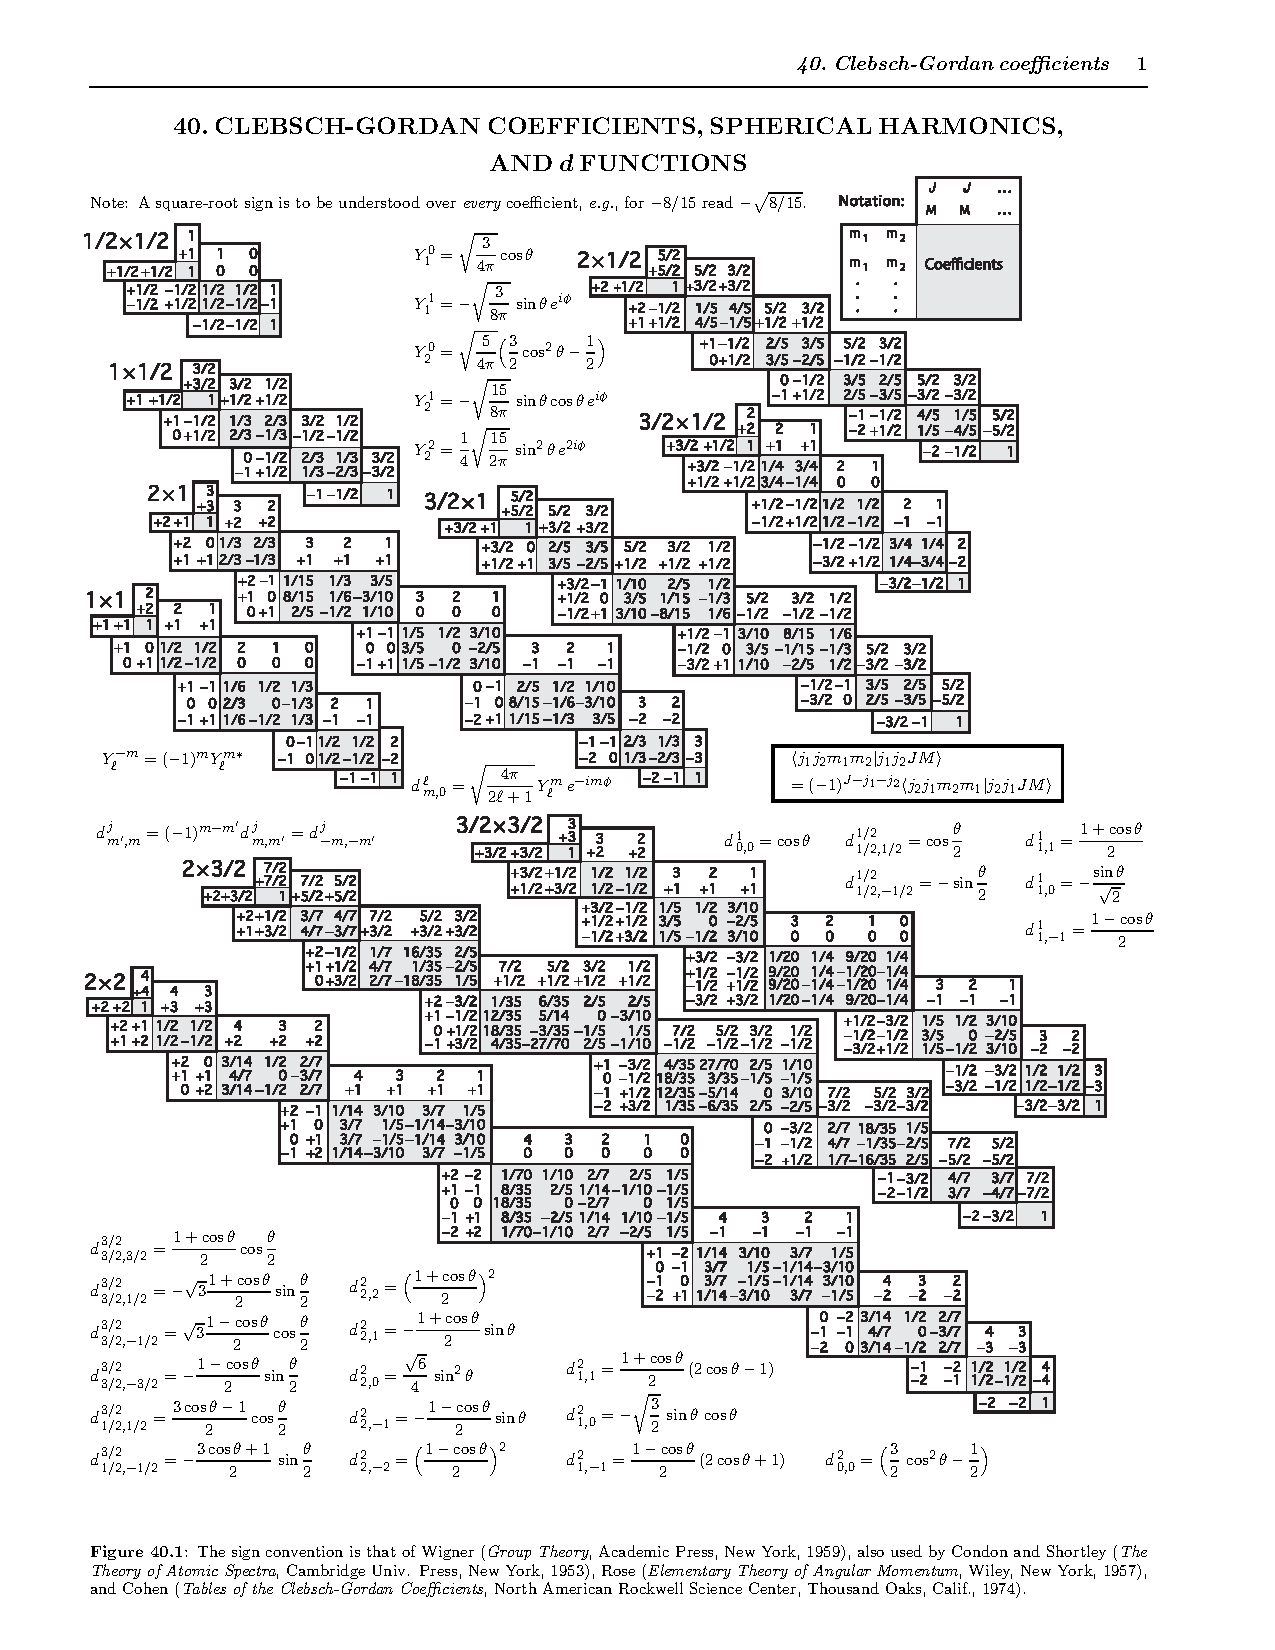
\includegraphics[height=0.9\textheight,keepaspectratio]{CGC}
    \caption{CCG}
    \label{fig:CCG}
\end{figure}
\end{frame}

\subsection{Densit\'a degli stati per N fermioni identici in una scatola}

\begin{frame}{Stati particella in scatola}
Density of available state $\frac{dN}{4\pi p^2dp}$ is given by $dN=4*\frac{4\pi p^2\Omega}{h^3}dp$: we are allowed to place 4 particles in each orbital (spin-isospin).

*Spazio delle Fasi
In un volume dello spazio delle fasi $(2\pi\hbar)^3$ ci stanno al pi\'u $\nu$ particelle dove $\nu$ \'e la degenerazione.

Density of states
Semi-Euristico (Numero di stati fratto volume dello spazio delgi impulsi):

Number of states between $p$ e $p+dp$ is given by $dN=4*\frac{d^3p}{(2\pi\hbar)^3}\Omega=4*\frac{4\pi p^2dp}{(2\pi\hbar)^3}\Omega$.

The infinitesimal thin spherical shell with radius $dp$ has the volume $4\pi p^2dp$.

$g(k)=\frac{dN}{4\pi p^2dp}=\nu\frac{\Omega}{(2\pi)^3}$.

*Stati particella in una scatola
Sia il numero di stati tra $n$ e $n+dn$: $dN=\nu \frac{4\pi n^2dn}{8}$, dove $\nu$ \'e il fattore di degenerazione. La densit\'a di stati fra $k$ e $k+dk$ \'e $g(k)=\frac{dN}{4\pi k^2dk}=\nu \frac{V}{(2\pi)^3}$.

$g(k)=\frac{dN}{4\pi k^2dk}=\nu \frac{V}{(2\pi)^3}$
    
\end{frame}

\begin{wordonframe}{ Density  states for N spin 0 particles in a box}
 
A particle state has volume $h$ in the phase space: we can count particle states as the total phase space volume accessible to that particle divided by the volume of a state. Considero una particella in un volume V (around the scattering center): il numero di stati con momento tra $\vec{p'}$ e $\vec{p'}+d\vec{p'}$ \'e $dn(|\vec{p'}|)=\frac{V*4\pi p^2}{h^3}dp'$ e ho $\rho(E')=\frac{dn(p')}{dE'}=\frac{dn(p')}{v'dp'}=\frac{V*4\pi p^2}{v' h^3}$


\end{wordonframe}

\subsection{Regola d'oro di Fermi}

\begin{frame}{Fermi's golden rule}
 
Probability of transition per unit time: $W_{i\rightarrow f}=\frac{2\pi}{\hbar}|\braket{f|H_{int}|i}|^2\rho(E')$, con $\rho(E')=\frac{dn(E')}{dE'}$.\\
Scattering rate per incident particle and per scattering center: \ev{W_{i\rightarrow f}=\frac{R_b}{N_aN_x}}, with the scattering rate $R_b=\Phi_a\sigma N_x$ ($\phi=n_av_a$): \ev{\sigma=\frac{2\pi}{\hbar v_a}|M_{fi}|^2\rho(E')V}.
Per stati d'onda piana \lbt{\psi_i=\frac{1}{\sqrt{V}}exp(\frac{i\scap{p}{r}}{\hbar})}{\psi_f=\frac{1}{\sqrt{V}}exp(\frac{i\scap{p'}{r}}{\hbar})}
    
\end{frame}


\section{Decadimenti,cinematica (e relativistica)}

\subsection{Decadimenti}

\begin{frame}{Energetica urti/decadimenti}
    \begin{itemize}
\item Equazioni relativistiche per particella $m_1$ incidente su bersaglio fermo $m_2$\\
$\Delta M=\sum_im_{(i)}-(m_1+m_2)$\\
\textbf{Energia CM/LAB}: $E_{cm}=\sqrt{{m_1}^2+{m_2}^2+2\epsilon_{1l}m_2}=\sqrt{({p_1}^{\mu}+{p_2}^{\mu})^2}$\\
\textbf{Energia di soglia nel CM}: ${E_c}^{th}=m_1+m_2+\Delta M$\\
\textbf{Energia di soglia nel Lab}: ${E_{1Lab}}^{th}-m_1=\underbrace{\delta M}_{(-Q)}[1+\frac{m_1}{m_2}+\frac{\Delta M}{2m_2}]$
\item Energia cinetica dei frammenti di un decadimento $\underbrace{A}_M\rightarrow \underbrace{a_1}_{m_1}+\underbrace{a_2}_{m_2}$, nel riferimento di quiete di M.

 Si conservano (c=1) \lbt{\text{Energia: }  M=m_1+m_2+T_1+T_2=e_1+e_2}{\text{Impulso: nel CM }  \vec{0}=\vec{p_1}+\vec{p_2}}
quindi $\underbrace{\vec{p_1}^2}_{e_1^2-m_1^2}=\underbrace{\vec{p_2}^2}_{e_2^2-m_2^2} (M=e_1+e_2) \Rightarrow$\lbt{e_1=\frac{M^2+m_1^2-m_2^2}{2M}}{e_2=\frac{M^2+m_2^2-m_1^2}{2M}}

\end{itemize}

\end{frame}


\section{Collisioni: scattering}

\begin{frame}{Sezione d'urto}
\begin{block}{Numero di urti in $dV$, $dt$.}
\begin{equation*}
    d\nu=\sigma v_{rel}n_1n_2\,dV\,dt
\end{equation*}

The luminosity measures the ability of a particles accelerator to produce the required number of interaction.
 $\# \text{eventi per unit\'a di tempo}=\mathcal{L}\sigma$:\\
$\mathcal{L}=\frac{\text{\# incident particles}}{\text{Area}*\text{Time}}*(\text{\# target particles})=\frac{\text{\# incident particles}}{\text{Time}}\frac{\text{\# target particles}}{\text{Area}}$(Il tutto \'e omogeneo).
\end{block}

\begin{block}{Differential cross section}
$\frac{d\sigma}{d\Omega}=\frac{\text{Events into solid angle $d\Omega$ at $(\theta,\phi)$ per unit time}}{d\Omega*(\text{Incident particles})*(\text{Target nuclei} per cm^2)}$.

Differential Probability of scattering by an angle $\theta$. For each nucleus the probability of scattering by an angle between $\theta$ and $\theta+d\theta$ is equal to the probability of the incident particle having an impact parameter between $b$ and $b+db$: $\frac{dP}{d\theta}d\theta=\frac{dP}{db}db=2\pi bdbN_x=(\text{area per nucleus})*(\text{nuclei per }cm^2)$
\end{block}
Connection between $\frac{d\sigma}{d\Omega}$ and $\frac{dP}{d\theta}$: $N_x\frac{d\sigma}{d\Omega}d\Omega=N_x\frac{d\sigma}{d\Omega}2\pi\sin{\theta}d\theta=\frac{dP}{d\theta}d\theta$.
\end{frame}

\begin{wordonframe}{Angoli Lab-CM (NR)}
    Relazioni sistema Lab ($m_2$ immobile) - sistema CM; $\vec{V}=\frac{m_1\vec{v_1}+m_2\vec{v_2}}{m_1+m_2}$.

Angoli: \lbt{\tan{\theta_1}=\frac{m_2\sin{\chi}}{m_1+m_2\cos{\chi}}}{\theta_2=\frac{\pi-\chi}{2}}.
Velocit\'a: \lbt{\vec{v_1}=\frac{m_2}{m_1+m_2}\vec{v}+\vec{V}}{\vec{v_2}=-\frac{m_1}{m_1+m_2}\vec{v}+\vec{V}}.

Velocit\'a dopo l'urto in Lab in funzione di $\chi$\\
Con $\vec{v}=\vec{v_1}-\vec{v_2}$: 
\lbt{v_1'=\frac{\sqrt{{m_1}^2+{m_2}^2+2m_1m_2\cos{\chi}}}{m_1+m_2}v}{v_2'=\frac{2m_1v}{m_1+m_2}\sin{\frac{\chi}{2}}}.

\end{wordonframe}

\begin{wordonframe}{Sezione d'urto}
$n=$ target atoms per unit volume, $\frac{\rho}{A}N_A$, con $A=$ mass number of target (pure isotope), $\rho x=$ areal density of target $(g/{cm}^2)$, $\rho=$ mass density of target (${g/{cm}^2}$), $nx=$ areal number density $nx=$ areal number density (atoms/$cm^2$) $=\frac{\rho}{A}xN_{Avogadro}$, con $x=$ thickness of target $(cm)$.

 Sia $dR_b$ il numero di particelle scatterate per unit\'a di tempo nell'angolo solido\\ $d\Omega=\sin{\theta} d\theta d\phi$, la sezione d'urto differneziale \'e data da:
 $d\sigma(\Omega)=\frac{dR_b}{I_aN_x}=\frac{1}{I_anx}*\mathcal{F}(\theta,\phi)*\frac{d\Omega}{4\pi}$ con $\int\mathcal{F}(\theta,\phi)\frac{d\Omega}{4\pi}=R_b$.
 
%$\frac{d\sigma}{d\Omega}d\Omega=\frac{\text{\# particelle diffuse per unit\'a di tempo in $d\Omega$}}{\text{\# particelle incidenti per unit\'a di area e di tempo}}$.
%Probabilit\'a che una particella $\alpha$ scatterata incida su un rilevatore di area $A_d$ ad angolo $\theta$: ${A_dN(\theta)}$ ($dN_b(\theta)=I_aN(\theta)A_d, \Delta \sigma=\frac{dN_b}{I_aN_x}$), rimuoviamo la dipendenza dalla geometria del rilevatore dividendo per $\Delta \Omega=\frac{A_d}{r^2}$.

\end{wordonframe}

\subsection{Rutherford scattering}

\begin{frame}{Scattering coulombiano}
Sezione d'urto differenziale per potenziale coulombiano (Formula di Rutherford)
$d\sigma=\pi(\frac{\alpha}{m{v_{\infty}}^2})^2\frac{\cos{\frac{\chi}{2}}}{\sin^3{\frac{\chi}{2}}}=(\frac{\alpha}{2m{v_{\infty}}^2})^2\frac{d\Omega}{\sin^4{\frac{\chi}{2}}}$.

Small deflection angle (region of closest approach: $\Delta x\approx 2b$, $\Delta t\approx\frac{2b}{v}$) The momentum transfer is nearly perpendicular to the incident momentum: $\Delta p_{\perp}\approx \overline{F_{\perp}}\Delta t$.

$\theta\approx\frac{\Delta p_{\perp}}{p}=\frac{2zZ\alpha}{pvb}$ (relativistic) which agrees with non-relativistic calculation $\frac{\theta}{2}\approx\tan{\frac{\theta}{2}}=\frac{zZ\alpha}{2bE_k}=\frac{zZ\alpha}{pvb}$.
Small angle approx: $\frac{d\sigma}{d\Omega}\approx(\frac{2zZ\alpha}{pv})^2\frac{1}{\theta^4}$. 
Frazione di particelle con parametro minore di $b_0$ $f_{b<b_0}=f_{\theta>\theta_0}=\frac{\rho N_A}{M}\pi b_0^2t$.
\end{frame}

\begin{wordonframe}{Scattering Rutherford}
 Scattering angle (small angle), scattering in potenziale coulombiano:
$U(r)=\frac{\alpha}{r}$, Coulomb force on the beam particles with mass $m$ and charge $ze$: $F=\frac{\alpha \hbar c zZ}{r^2}$.

Traiettoria particella $\alpha (ze)$ scatterata da un nucleo $(Ze)$:
$\frac{1}{r}=\frac{1}{b}sin{\phi}+\frac{(ze)(Ze)}{8 \pi \epsilon_0Kb^2}(cos{\phi}-1)$, $K$ energia cinetica della particella $\alpha$ espressa in $eV$ quindi $b=\frac{(ze)(Ze)}{8 \pi \epsilon_0K}cot{\frac{\theta}{2}}$.

\end{wordonframe}

\begin{wordonframe}{Relativistic corrections}

Relazione mass shell: $pc=\sqrt{E^2-(mc^2)^2}$.

Rinculo del nucleo M:
Trascurando la massa $m_e$ dell'elettrone dalla conservazione del 4-momento ho $EMc^2=E'E-\scap{p}{p'}c^2+E'Mc^2$ quindi per l'energia dell'elettrone dopo l'urto $E'=\frac{E}{1+\frac{E}{Mc^2}(1-\cos{\theta})}$.

CEM of a moving charge ($\vec{R}=(X-vt,Y,Z)$) Electric field along direction of motion: $E_{//}=\frac{e}{4\pi\epsilon_0R^2}(1-\frac{v^2}{c^2})$.

Electric field perpendicular to the direction of motion: $E_{\perp}=\frac{e}{4\pi\epsilon_0R^2}\frac{1}{(1-\frac{v^2}{c^2})^{\frac{1}{2}}}$.

Relativistic correction to EM strenght: In the frame of moving particle the EF in trasverse direction is multiplied by $\gamma$ and in compressed by same factor into a smaller region along the direction of particle motion: $\Delta p_{\perp}\approx\frac{\alpha zZ[\gamma]}{b^2}\frac{2b}{v[\gamma]}$.
\end{wordonframe}


\begin{frame}{Scattering qm}
    \begin{columns}[T]
\begin{column}{0.5\textwidth}
\begin{figure}
    \centering
    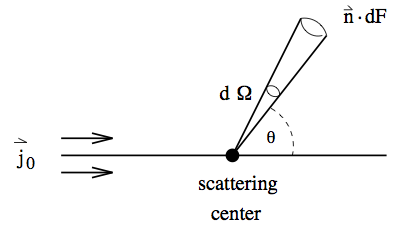
\includegraphics[scale=0.2]{ds}
    \caption{Scattering center: geometry}
    \label{fig:scatgeom}
\end{figure}
\end{column}
\begin{column}{0.5\textwidth}
In termini QM: From the incoming current $\vec{j}_0$ of particles the scattering process create a current $\vec{j}^{sc}$ of scattered particles, $d\sigma=\frac{\vec{j}^{sc}\cdot\hat{n}dF}{|\vec{j}_0|}=\frac{\vec{j}^{sc}\cdot\hat{n}r^2d\Omega}{|\vec{j}_0|}$.
\end{column}
\end{columns}
Soluzione generale per scattering elastico \'e:
 $\braket{\vec{x}|\psi^{\pm}}=\underbrace{\braket{\vec{x}|\phi}}_{\text{onda incidente}}-\underbrace{\frac{2m}{\hbar^2}\int d^3x'\frac{e^{\pm k|\vec{x}-\vec{x'}|}}{4\pi|\vec{x}-\vec{x'}|}\braket{\vec{x'}|V|\psi^{\pm}}}_{\text{Effetto della diffusione}}$.
\end{frame}

\begin{wordonframe}{Scattering ampiezza probabilit\'a}
Lunghezza d'onda di de Broglie: $\lambda=\frac{2\pi \hbar}{p}=\frac{2\pi c\hbar}{pc}=\frac{2\pi (\hbar c)}{\sqrt{E^2-(mc^2)^2}}$.

$\lambdabar=\frac{1}{k}$, $\hbar c\approx 197.3 MeV*fm$.

Optically resolvible object:
per risolvere un oggetto di dimensione caratteristica d con fascio di particelle di lunghezza d'onda $\lambda$ devo avere $\lambda\ll d$.

Corrente di  probabilit\'a: onda piana e funzione d'onda di scattering.

\textbf{Per un'onda piana}: $\vec{J_0}=\frac{\hbar}{m}\Im{[\frac{e^{-\frac{i}{\hbar}\scap{p}{x}}}{(2\pi\hbar)^{\frac{3}{2}}}\nabla(\frac{e^{\frac{i}{\hbar}\scap{p}{x}}}{(2\pi\hbar)^{\frac{3}{2}}})]}=\frac{\frac{p}{m}}{(2\pi\hbar)^3}$\\
\textbf{Per un'onda sferica (scattered wave)}: $\vec{j}^{sc}=|\psi^{sc}|^2v'\hat{n}$.
de Broglie wavelength: $\lambda$ ($\lambdabar=\frac{1}{k}$)\\
$\frac{\lambda}{2\pi}=\frac{\hbar}{p}=\frac{\hbar c}{\sqrt{2mc^2E_{\text{kin}}+E_{\text{kin}}^2}}\approx$\lbt{\frac{\hbar}{\sqrt{2mE_{\text{Kin}}}}\text{ , } E_{\text{Kin}}\ll mc^2}{\frac{\hbar c}{E_{\text{Kin}}}\approx\frac{\hbar c}{E} \text{ , }E_{\text{Kin}}\gg mc^2}.
Cross section:
$\frac{d\sigma}{d\Omega}=(\frac{\overbrace{\alpha}^{(ze)(Ze)}}{4E_{\text{Kin}}})^2\frac{1}{\sin^{\frac{\theta}{2}}}$\\
Per velocit\'a relativistiche:\\
$(\frac{d\sigma}{d\Omega})_{\text{Mott}}=(\frac{d\sigma}{d\Omega})_{\text{Ruth}}(1-\beta^2\sin^2{\frac{\theta}{2}})\abl{v}{c}(\frac{d\sigma}{d\Omega})_{\text{Ruth}}\cos^2{\frac{\theta}{2}}$.\\
Suppression of backscattering ($\theta=\pi$) for target with spin 0 it's a consequence of conservation of helicity.
\end{wordonframe}

\begin{wordonframe}{scattering}
 Urto elastico:
 $H_0\ket{\phi}=E\ket{\phi}. (H_0+V)\ket{\psi}=E\ket{\psi}$, $H=H_0+V, H_0=\frac{\vec{P}^2}{2m}$: in assenza di un centro diffusore, $V=0$, gli autostati sono quelli di $\ket{\vec{P}}$,  per $V\neq0$ gli autostati dell'energia $\neq \ket{\vec{P}}$ tuttavia se il processo d'urto \'e elastico siamo interessati alla soluzione dell'ES per l'hamiltoniana completa con la stessa energia.

Operatore densit\'a di corrente:
Sommo il contribiuto delle funzioni d'onda di tutti i protoni:\\
$\sum_{i=1}^Z|\psiN{Z}|^2\frac{e}{m}\vec{p_i}d^3x_1\ldots d^3x_Z$,\\
 l'integrale \'e su tutte le coordinate eccetto la i-esima e l'elemento della sommatoria relativo \'e il contributo alla corrente dell'i-esimo protone.

\end{wordonframe}

\begin{frame}{Scattering: centro non puntiforme}
    
     \begin{itemize}

\item Born Formula\\
$\frac{d\sigma}{d\Omega}=(\frac{m}{2\pi\hbar^2})^2|\int U(r)e^{i(\vec{k}-\vec{k'})\cdot\vec{x}}d^3x|^2$


\item  Fattore di forma\\
$-Ze^2\int d^3x\int d^3x'\frac{N(r')e^{i\vec{q}\vec{x}}}{|\vec{x}-\vec{x'}|}=Ze^2\frac{4\pi}{q^2}F(\vec{q})$, con \ev{ F(\vec{q})=\int d^3x' e^{i\scap{q}{x'}}N(x')}.

Espansione di $e^{i\scap{q}{x}}$ per piccoli q:
$e^{i\scap{q}{x}}=1+i(\vec{k}-\vec{k'})\cdot\vec{x}-\frac{[(\vec{k}-\vec{k'})\cdot\vec{x}]^2}{2}+\ldots$

Espressione integrale potenziale Coulombiano (Approx. grandi distanze).

\input{coulombdistant}




 \end{itemize}

\end{frame}

\begin{wordonframe}{Scattering di particelle}
 
Sviluppi asintotici:
Per $r=|\vec{x}|\gg r'=|\vec{x'}|$: $e^{\pm ik|\vec{x}-\vec{x'}|}\approx e^{\pm ikr}e^{\mp ik\hat{r}\cdot\vec{x'}}$\\
$\frac{1}{\vec{x}-\vec{x'}}\approx\frac{1}{r}$\\
$|\vec{r}-\vec{r'}|\approx r-\hat{r}\cdot\vec{r'}$\\
In particolare: $\isw{k}{|\vec{r}-\vec{r'}|}\approx\isw{k}{r}e^{-ik\hat{r}\cdot\vec{r'}}$.

Integrale utile per il fattore di forma del potenziale di Yukawa
$\Im{\int_0^{\infty}e^{-\mu r}e^{iqr}dr}=\frac{q}{\mu^2+q^2}$.

FT di $\frac{1}{r}$,
$\int d^3x\frac{e^{i\scap{q}{x}}}{|\vec{x}|}=\frac{4\pi}{q^2}$\\
$\nabla^2\frac{1}{r}=-4\pi\delta^3(\vec{r})$ in trasformata di Fourier diventa $-\vec{q}^2FT(\frac{1}{r})=-4\pi$.

Potenziale come convoluzione: Nel caso il potenziale scatteratore non sia genarato da una carica puntiforme  ma da una distribuzione di carica $\rho(\vec{r})$  il potenziale \'e dato dalla convoluzione $U=\rho\star\frac{1}{r}$.

Impulso trasferito: $q=\frac{2E}{\hbar c}\sin{\theta}{2}$

Esponenziale: $\exp{(\frac{i\scap{q}{r}}{\hbar})}=\sumzi{n}\frac{1}{n!}(\frac{iqr\cos{\theta}}{\hbar})^n$

RK: $E\gg mc^2\Rightarrow E\approx|\vec{p}|c$

\end{wordonframe}

\section{Fisica atomica}


\subsection{Alkali}

\subsection{Helium}

\subsection{Vectorial model}

\part{Interazioni fondamentali, particelle (/mediatori), modello standard}\linkdest{SM}
\begin{wordonframe}{Standard model}
\begin{itemize}
\item Scattering: Rutherford,etc
\item Interazioni fondamentali
\item Interazioni forti: ipotesi di yukawa
\item parit\'a intrinseca \Ppi
\item Interazioni deboli
\item Decadimenti
\item Isospin: scattering pp, processi \Ppi-N
\item Leptoni, mesoni, barioni, quarks
\item stranezza, etc
\item Elettrone relativistico: rappresentazione di Bjorken-Drell
\item Precessione spin in campo magnetico, forza di Lorentz, precessione di Thomas
\item Equazione di Dirac.
\item Antimateria
\item Propriet\'a sistemi particelle identiche sotto scambio
\item Livelli energetici in potenziale coulombiano: positronio, quarkonio
\item Supersimmetria
\item Elicit\'a
\item Operatore parit\'a
\item Generalizzazione principio di Pauli
\item Diagrammi di Feynmann
\item Simmetria CP
\item momento magnetico e momento angolare
\item r4elazione energia-momento angolare delle particelle
\item Operatore C, G-parit\'a
\item Simmetrie: $U(1)\times SU(2)\times SU(3)$, T. di Noether
\item Teorema CPT (Schwinger, Luders, Pauli)
\item Neutrini di Dirac/Majorana
\item fenomeni di oscillazione in fisica delle particelle: differenze di massa ed elementi non diagonali in H
\end{itemize}
\end{frame}
\input{forcesparticles}

\part{Leptons}\linkdest{leptons}
\begin{wordonframe}{Leptoni: neutrini, elettroni, etc}
\begin{itemize}
\item Elettrone/positrone:
\item Moto spin in campo magnetico (BMT, precessione anomala)
\item Misura (g-2)
\item Ipotesi di Pauli del neutrino
\item famiglie leptoniche e relazione con famiglie di quarks
\item Exp Reines-Cowan 55: rivelazione anti-nu da reattore. Exp Davis; exp BNL-Columbia
\item Exp di Goldhaber su elicit\'a neutrino
\item Limiti alla massa del n eutrino dal decadimento beta del trizio 
\item oscillazioni neutrini
\item positronio; exp di deutsh 51
\item g-2
\end{itemize}
\end{wordonframe}
\input{leptons}

\part{Quarks}\linkdest{quarks}
\begin{itemize}
\item cinematica dei decadimenti
\item scoperta muone/pione
\item Esperimento di Bryman
\item risonanze
\item teta-tau puzzle, ipotesi di Yang-Lee, esperimento di Wu (articoli: Lee-yang, Wu, Lederman)
\item particelle strane: sistemi K. Mesoni $K_S$, $K_L$ autostati di CP  parit\'a.
\item esperimento di cronin
\item violazione parit\'a in interazioni deboli
\item produzione particelle strane; rivelazione neutrini
\item produzione Y* (Alston 60)
\item decadimento K0/K0bar
\item Basi ortonormali per descrivere K
\item Esperimento di Carithers75: interferenza nello stato finale a 2 pi provenienti da KS e KL
\item Valore costante debole di Fermi: decadimento mu, decadimento N e decadimento Sigma; ipotesi di Cabibbo63: AS delle WI sono una classe degli AS delle SI.
\item Ipotesi GIM: esistenza 4o quark 1970.
\item Ipotesi Kobayashi-Maskawa 72
\end{itemize}
\end{frame}
\input{quarks}

\part{produzione adroni e leptoni pesanti}\linkdest{hhlfactories}
\begin{wordonframe}{Produzione adronica: acceleratori}
\begin{itemize}
\item Produzione adronica: ee, vector boson dominance, quarto/quinto quark, Y(9460)
\item  Sezione d'urto e+e- to mumu
\item Misura larghezza risonaqnze strette
\item Scoperta del quark c; exp richter (pear); exp Ting (BNL). Conferma meccanismo GIM per J/psi.
\item scoperta leptone tau
\item scoperta quark b
\item produzione di jets in e+e-
\item esistenza del colore
\item running constant
\item regola di OZI

\end{itemize}
\end{wordonframe}
\input{hhlfactories}

\part{Crucial experiments}
\begin{frame}{this part toc}
\begin{itemize}
\item Wu(1957)
\end{itemize}
\end{frame}
\begin{wordonframe}{}

\end{wordonframe}


\part{List of sorted keywords}


\end{document}